\documentclass[11pt,dvipdfmx]{jreport}
\usepackage{wuse_thesis}
\usepackage{indentfirst}
\usepackage{url}	% \url{}コマンド用.URLを表示する際に便利
\usepackage{graphicx}  % ←graphicx.styを用いてEPSを取り込む場合有効にする
\usepackage{color}
 \usepackage{multirow} 
\newcommand{\todo}[1]{\colorbox{yellow}{{\bf TODO}:}{\color{red} {\textbf{[#1]}}}}
%\usepackage{graphicx}  % ←graphicx.styを用いてEPSを取り込む場合有効にする
			% 他のパッケージ・スタイルを使う場合には適宜追加

%%%%%%%%%%%%%%%%%%%%%%%%%%%%%%%%%%%%%%%%%%%%%%%%%%%%%%%%%%%%%%%%%%%%%%%%

%%
%% 主に表紙を作成するための情報
%%

%%  タイトル(修論の場合は英語表記も指定)
\title{Scratchにおける学習者の作品制作過程に基づく\\
コンピュテーショナル・シンキング習熟度の\\
到達予測}
%\etitle{Test\\Test\\Test}

%%  著者名(修論の場合は英語表記も指定)
\author{岡本 圭悟}
%\eauthor{Akinori Ihara}

%% 卒業論文・修士論文(以下のどちらかを選択)
\bachelar	% 卒業論文(4年生用)
%\master  	% 修士論文(M2用)

%%  学科・クラスタ
\department{システム工}
%\department{デザイン情報}
%\department{デザイン科学}

%%  学生番号
\studentid{60256053}

%%  卒業年度
\gyear{2023}		% 提出年が2022年なら,2021年度

%%  論文提出日
\date{2024年2月13日}	% 修士の場合は月(2021年2月)までとし,英語表記も指定
%\edate{February 2021}	% 修士の場合,こちら(英語表記)も有効化

%%%%%%%%%%%%%%%%%%%%%%%%%%%%%%%%%%%%%%%%%%%%%%%%%%%%%%%%%%%%%%%%%%%%%%%%

\begin{document}

\maketitle

%%
%%  概要
%%
\begin{abstract}
本研究では,Scratchにおけるユーザのコンピュテーショナル・シンキング(CT)の作品制作過程に合わせた作品推薦に向けて,ユーザが予測時点でCT習熟度が向上する作品を制作するか否かを予測する手法を提案する.

Scratchでは,ユーザが命令処理を持つ視覚的に表現されたブロックを組み合わせてプログラムを実装し,作品制作を通してプログラミング学習の目的であるCTを身につける.特に,ユーザは学習支援ツールDr.Scratchを使用することで,制作した作品のプログラムを基に7つの概念でそれぞれCTスコアが計測され,自身のCTスキルを定量的に把握できる.

従来研究では,ユーザが過去に獲得した7つのCT概念の点数結果から,CTスコア合計点の区分であるCT習熟度への到達可否を予測するモデルを構築,評価した.しかし,従来モデルでは異なる作品制作過程を経ているユーザでも,同じCTスコアの場合は予測結果が同じになってしまうことから,ユーザの作品制作過程は十分考慮できておらず誤って予測することがある.このことから作品制作過程を考慮したモデルを構築することで,従来モデルで予測できなかった作品制作過程が類似するユーザの習熟度到達予測が可能になると考える.

本研究は,Scratchにおけるユーザの作品制作過程に合わせた作品推薦に向けて,まずユーザの作品制作過程の特徴を把握するためにユーザが獲得してきたCT7概念の特徴量を分析した.さらに,ユーザが獲得してきたCT7概念を説明変数とした学習モデルを作成し,予測,従来モデルとの比較評価を行った.分析の結果,ユーザが獲得してきたCT概念の獲得過程には特徴があり,CT概念の獲得過程を考慮した説明変数としたモデルを構築することで従来モデルよりも精度が向上することが示唆された.本研究により,Scratchにおけるユーザの成長過程に合わせた学習支援の役立てとなることを期待する.

\end{abstract}

%%  目次
\tableofcontents

%%  図目次 (図目次をいれたければ以下のコメントをはずす)
%\listoffigures

%%  表目次 (表目次をいれたければ以下のコメントをはずす)
%\listoftables

\newpage
\pagenumbering{arabic}	% 以降のページ番号を算用数字に

%%%%%%%%%%%%%%%%%%%%%%%%%%%%%%%%%%%%%%%%%%%%%%%%%%%%%%%%%%%%%%%%%%%%%%%%

%%
%%  本文はここから
%%

\chapter{はじめに}
%%%%%%%%%%%%%%%%%%%%%%
近年,プログラミング教育は初等教育段階から導入されており,プログラミング教材の一つとして,MITメディアラボの開発するビジュアルプログラミング言語であるScratch~\cite{Resnick_2009}が利用されている.Scratchでは,プログラミングにおける命令処理を視覚的なブロックとして表現し,それらを組み合わせることでユーザの直感的なプログラム制作を実現している.また,ScratchはWeb上にオンライン学習サービス\footnote{Scratch: \url{https://scratch.mit.edu/}}を展開しており,ユーザは自身の制作した作品をサービス上に公開することで他ユーザが作品を参照することが可能である.サービスにはこれまでに多くの作品が公開されており,2024年1月15日時点で95,000,000件以上の作品が公開されている.

プログラミング学習の目的は,プログラミングの実装を通してコンピュテーショナル・シンキング(CT)~\cite{Wing_2006}を身につけることにある.CTとはプログラミングの問題に対する抽象的な分析や,その問題を解決するための効率的な考え方の総称であり,主に問題を応用可能な一般式にする抽象化,問題を一般式に当てはめて表現する実装,問題を解いて確かめる分析の3手順の反復によって習熟していく.Scratchにおいてもプログラムの命令処理の結果がスプライトの動きとして出力されるため,作品制作のプログラム実装を通してCTを身につけることができる.

ユーザが身につけたCTを把握するには,プログラムの実装内容を解析する必要があるため,プログラミング初学者にとって自身のCTを把握することは困難である.Scratchを用いたプログラミング学習を支援するツールとして,Morenoらはユーザが制作した作品に必要なCTを評価するDr.Scratch~\cite{Moreno_2015}を開発している.Dr.Scratchは,Scratch作品で利用されたブロックやプログラムの構造から作品の機能実装に必要な7つのCT概念をそれぞれ0点から3点までで算出し,合計点数0点から21点までの22段階で作品を評価する.特に,CTスキルの区分としてCT習熟度が存在し,0点から7点をBasic,8点から14点をDeveloping,15点から21点をMasterとしている.

従来研究として安東ら~\cite{Ando_2021}はユーザのCTに合わせた作品推薦に向けて,ユーザが過去に制作した作品のCTスキルに基づいてユーザが次にCT習熟度が向上するかを予測する研究を行なった.しかし,従来モデルでは異なる作品制作過程を経ているユーザでも,同じCTスコアの場合は予測結果が同じになってしまうことから,ユーザの作品制作過程は十分考慮できておらず誤って予測することがある.このことから作品制作過程を考慮したモデルを構築することで,従来モデルで予測できなかった作品制作過程が類似するユーザの習熟度到達予測が可能になると考える.

本研究では,ユーザのCTスキルの獲得過程に合わせた作品推薦に向けて,2つのResearch Question(RQ)に回答する.

\begin{description}
\item [RQ1:]CT習熟度が向上したユーザが獲得してきたCT7概念の違いはどの程度か?
\item [RQ2:]ユーザが獲得してきたCT7概念から次の作品でCT習熟度が向上するかどうかを予測することは可能か?
\end{description}

RQ1ではScratch作品の制作過程でCT習熟度が向上したユーザに着目して,各ユーザのCT7概念の獲得過程(CTパス)の特徴量を分析し,ユーザのCTパスの特徴,ユーザのCT概念の獲得過程に意味があるかを確認する.RQ2では学習者のCT7概念の獲得過程を考慮した学習支援のため,ユーザのCTスコア獲得過程を説明変数として学習モデルを作成し,ユーザが特定の習熟度に到達するか否かの予測を行い,従来モデルとの比較評価を行う.

以降,本論文では,2章で本論文の対象であるビジュアルプログラミング環境Scratchとそれに関連する従来研究
,本研究の位置づけを述べ,3章,4章では,設定したRQにおけるそれぞれの提案手法と結果,考察を述べる.続く5章では,妥当性の脅威を述べ,最後に6章で本論文をまとめる.

%杉浦学,松澤芳昭,岡田健,大岩元.アルゴリズム構築能力育成の導入教育:実作業による概念理解に基づくアルゴリズム構築体験とその効果.情報処理学会論文誌,Vol.49,No.10,pp.3409-3427,2008.
%森秀樹, 杉澤学, 張海, 前迫孝憲.Scratchを用いた小学校プログラミング授業の実践 : 小学生を対象としたプログラミング教育の再考(教育実践研究論文).日本教育工学論文誌,Vol.34, No.4, pp.387\UTF{2013}394, 2011.

% Scratchでは,ユーザは制作したプログラム作品にタイトルや作品の説明文を付けてScratchのオンラインサービス上に公開することができ,2023年7月時点には1億3500万件\footnote{Scratch Statistics: \url{https://scratch.mit.edu/statistics/}}以上の作品が公開されている.Scratchは公開済みの作品を対象に自然言語による作品検索サービスを提供しており,公開済み作品の中からユーザが制作したい作品,実現したい動作を検索し,実装の参考にしている\cite{Resnick_2009}.
% %Mitchel Resnick, John Maloney, Andr´es Monroy-Hern´andez, Natalie Rusk, Evelyn Eastmond, Karen Brennan, Amon Millner, Eric Rosenbaum, Jay Saul Silver, Brian S Silverman, Yasmin Bettina Kafai, Scratch: Programming for all, Communications of the ACM, Vol.52, No.11, pp.60-67, 2009.
% Scratchで制作する作品は小規模なプログラムが多く,使用するブロックも限られているため,検索によって類似するプログラムを含む作品が多数出力される.その一方で,プログラムは類似していてもオブジェクトの動作が異なることもある.このようなプログラムの類似性とオブジェクト動作の類似性の乖離は,Scratch上のプログラミング検索における作品の収集の妨げになることが示唆される.

% 本研究は,Scratchにおけるプログラムが類似する作品とオブジェクトの動作軌跡が類似する作品の違いを分析するために,Scratchにおいて制作されるプログラムの類似度の計測方法,およびオブジェクトの動作軌跡の類似度の計測方法を提案する.プログラムの類似度の計測方法にはプログラムの編集距離を用いる(3章).オブジェクトの動作軌跡の類似度の計測方法には動的時間伸縮法(DTW: Dynamic time warping)を用いる(3章).本研究では,ケーススタディとしてScratchAPIを用いて時系列順に収集し,条件に基づいてフィルタリングした4,000件の作品を対象に,プログラムが類似するか否か,オブジェクトの動作軌跡が類似するか否かの4種類に分類し,それぞれの作品の特徴を分析する.

% 続く\ref{sec:RelatedWork}章では本論文の立ち位置を説明するための関連研究と研究動機を述べる.\ref{sec:Similarity}章では本論文で用いる類似度の測定手法を述べる.\ref{sec:Analysis}章ではケーススタディで用いるデータセットとアプローチ,その結果と考察を述べ,\ref{sec:con}章で本研究をまとめる.

\chapter{Scratchを用いたプログラミングの学習環境}
\section{ビジュアルプログラミング言語Scratch}
ビジュアルプログラミングはプログラミング初学者がプログラミング的な思考を身につけるために視覚的なオブジェクトを操作して行うプログラミングの総称である.ScratchはMITメディアラボが開発するビジュアルプログラミング言語の開発環境であり,Scratchのユーザはプログラムの命令処理を持つ視覚的なブロックを組み合わせ,実行画面内のキャラクターの移動や効果音の入出力などをプログラムで制御することによりゲームやアニメーションなどの作品を直感的に制作できる.ScratchはC言語やJava言語等のテキストベースのプログラミングにおけるユーザの文字入力を必要としないためテキスト入力や構文によるエラーが発生しない.その結果,Scratchはテキストベースのプログラミング言語に比べて学習の難易度が比較的低く,教育現場でプログラミング初学者の学習ツールとして利用されることが多い.従来研究では,Scratchを用いたプログラミング学習の効果を確認し,Scratchを利用することでテキストベースのプログラミングへの移行を容易にすることが明らかとなった~\cite{Weintrop_2017}.
図\ref{fig:scratch-description}は,Scratch3.0における作品制作画面を示す.図\ref{fig:scratch-description}に示すように,Scratchにおけるプログラム作品は主にブロック,スクリプト,スプライトの3つの要素で構成される.
\begin{description}
\item [ブロック:]プログラムを構成する最小の単位であり,それぞれ特定の命令処理を持つ.ユーザは図\ref{fig:scratch-description}に示すようなブロックを組み合わせることでプログラムを実装する.Scratchでは,画像の移動を制御する座標移動ブロック,条件分岐や繰り返しなどの制御ブロックなどを提供しており,種類に応じて役割,色,形が異なり,Scratch3.0時点では全部で6種類の異なる形状のいずれかに分類される205種類のブロックが提供されている.表\ref{fig:scratch-description}は,6種類のブロックの形状それぞれの名称とその役割を示す.
\item [スクリプト:]図\ref{fig:scratch-description}に示すように複数のブロックを組み合わせて制作したプログラムを指す.特に,スクリプトの先頭にはプログラムを開始するイベントブロックを使用し,スクリプトを開始するためのトリガーを設定する.スクリプトはイベントブロック以降に配置されたブロックの命令処理を上から順に実行する.また,同じイベントブロックを持つスクリプトが並列に存在する場合は,同時にスクリプトを実行開始することができる.
\item [スプライト:]図\ref{fig:scratch-description}に示すように作品中に使用するキャラクターをはじめとした画像オブジェクトを指す.図\ref{fig:scratch-description}の作品では猫の画像オブジェクトがスプライトに該当する.また,各スプライトには,必ず一つ以上のスクリプトが紐づいており,スプライトを複数作成することも可能である.スプライトは実行画面上で,スクリプトに含まれる命令処理の通りに動作する.
\end{description}

図\ref{fig:scratch-description}に示す作品例は,緑の旗のイベントブロックを押下したときに,猫のスプライトが「こんにちは」と発言し,その後スプライトの向いている方向に10歩移動する動作を10回だけ繰り返す作品である.この事例のように,Scratchにおける作品はイベントブロックから始まり,スプライトの動作やメッセージを出力するスクリプトを1つのスプライトに対して1つ以上実装することで制作される.また,Scratchで制作した作品はオンラインサービス上に公開することができる.2023年1月時点で,1億人以上のユーザがScratchサービスにアカウント登録を行なっており,これまでに1億2千件以上の作品が公開されている.ユーザは他者が制作した公開作品の実装方法を容易に閲覧できるため,他者の作品を参照することで多様な実装方法を学習することができる.\cite{spfa}また,Scratchは他者の作品を基に自由にプログラムを書き換えることができるリミックスという機能を提供しており,この機能を用いてユーザはより多様なプログラムを参考にプログラム制作を行うことができる.本研究ではリミックスによって制作された作品をリミックス作品,ユーザが自身で一から制作した作品をオリジナル作品として区別する.

%--------------------

\begin{figure*}[t]
	\centering
	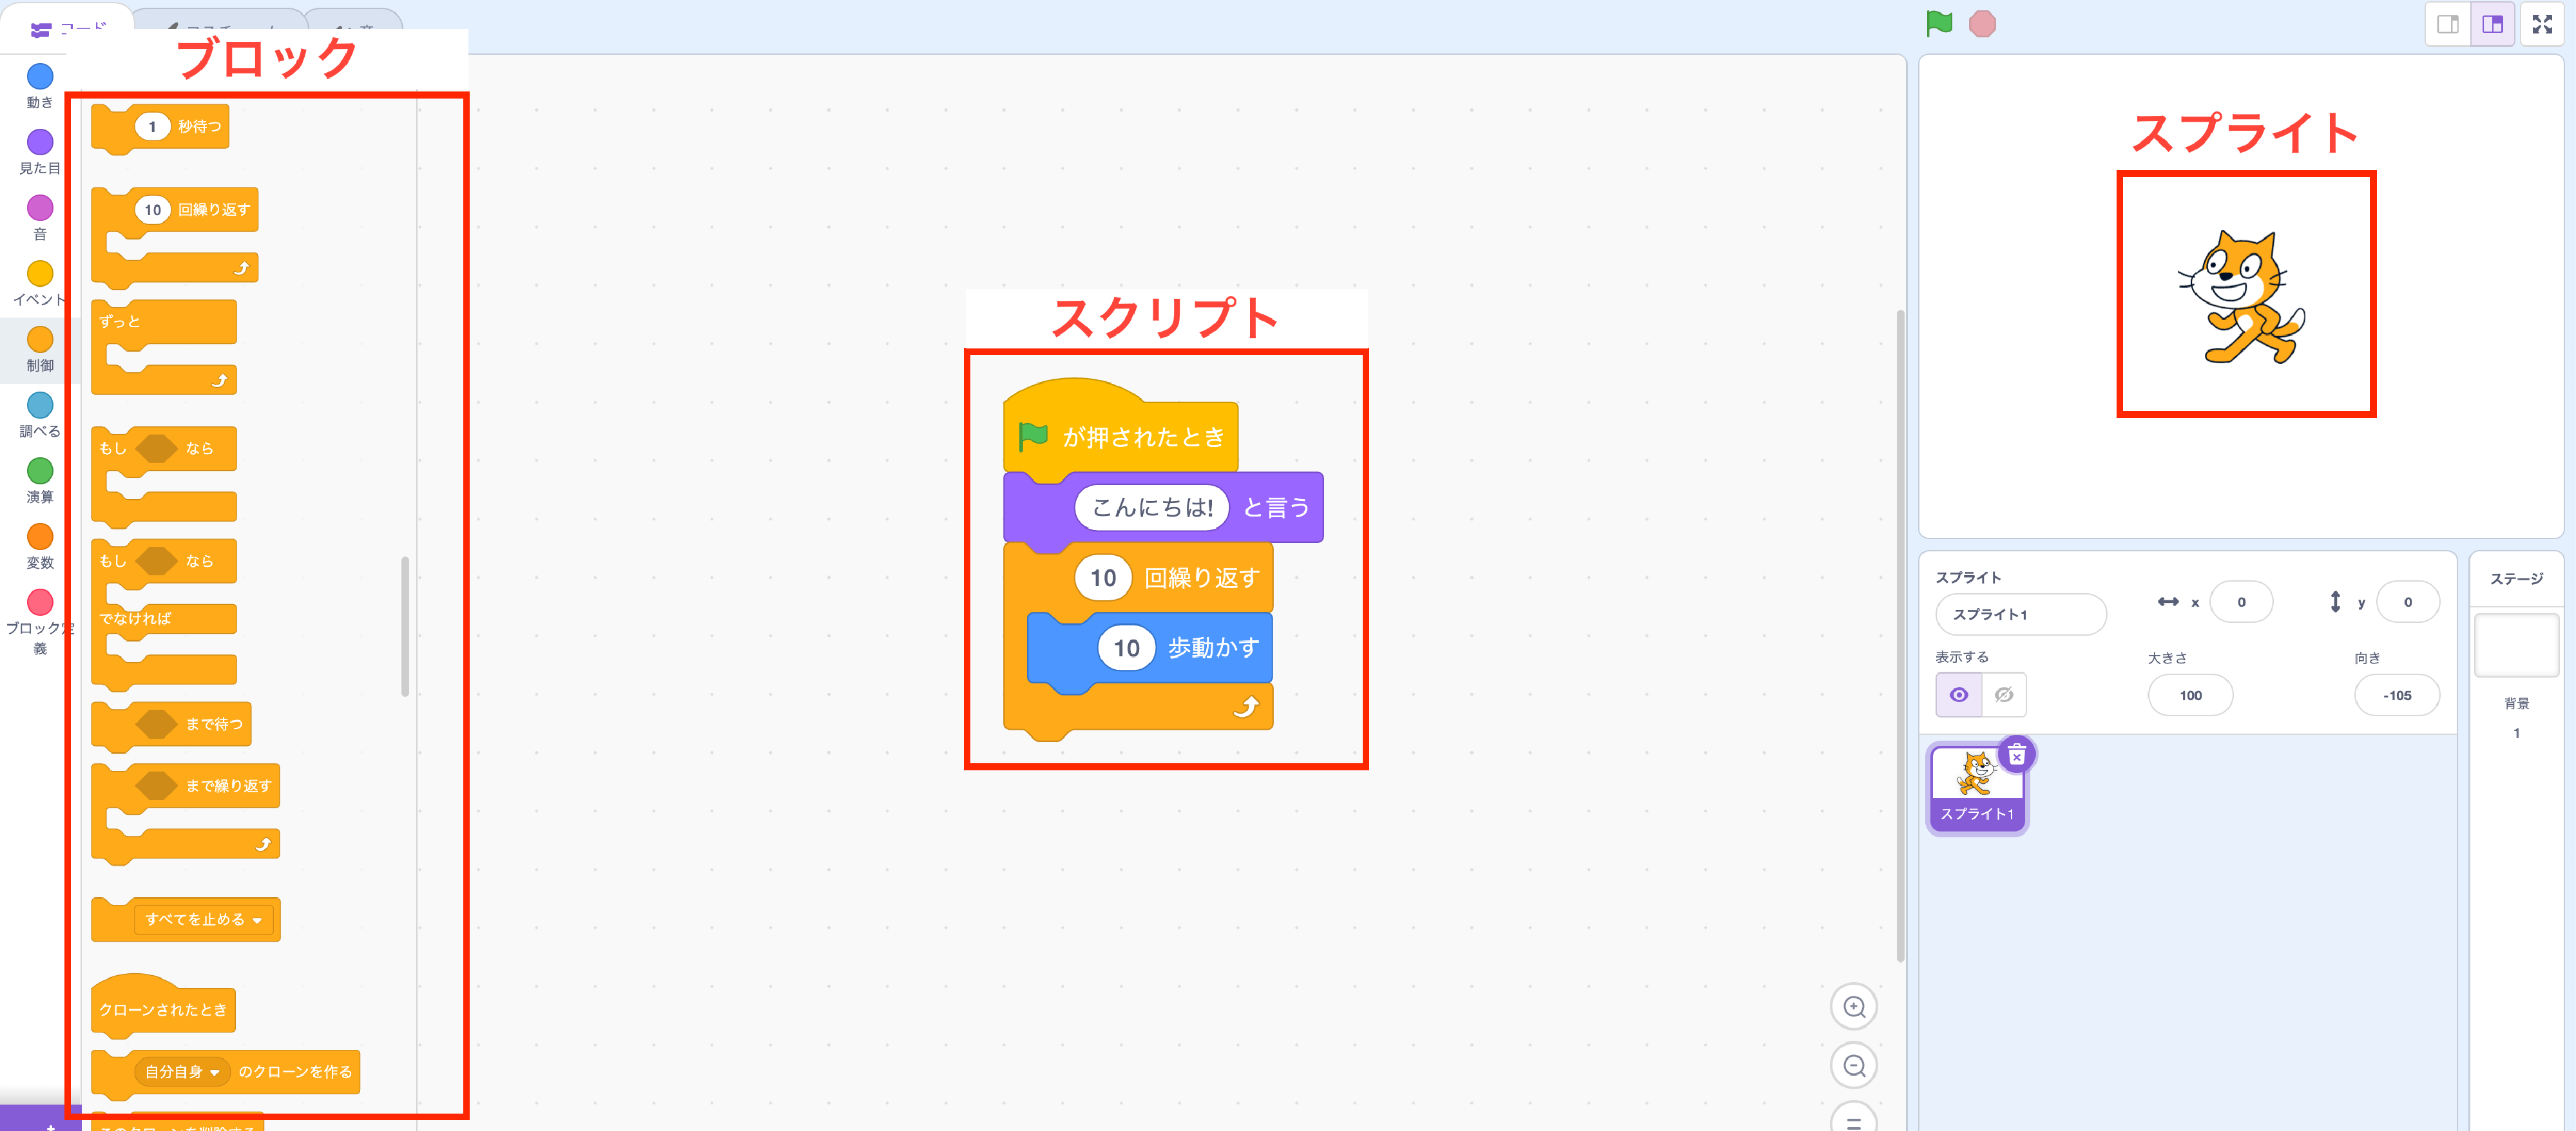
\includegraphics[width=0.9\linewidth]{Okamoto_fig/scratch-description.pdf}
	\caption{Scratchの作品制作画面}
	\label{fig:scratch-description}
\end{figure*}

\begin{figure*}[t]
	\centering
	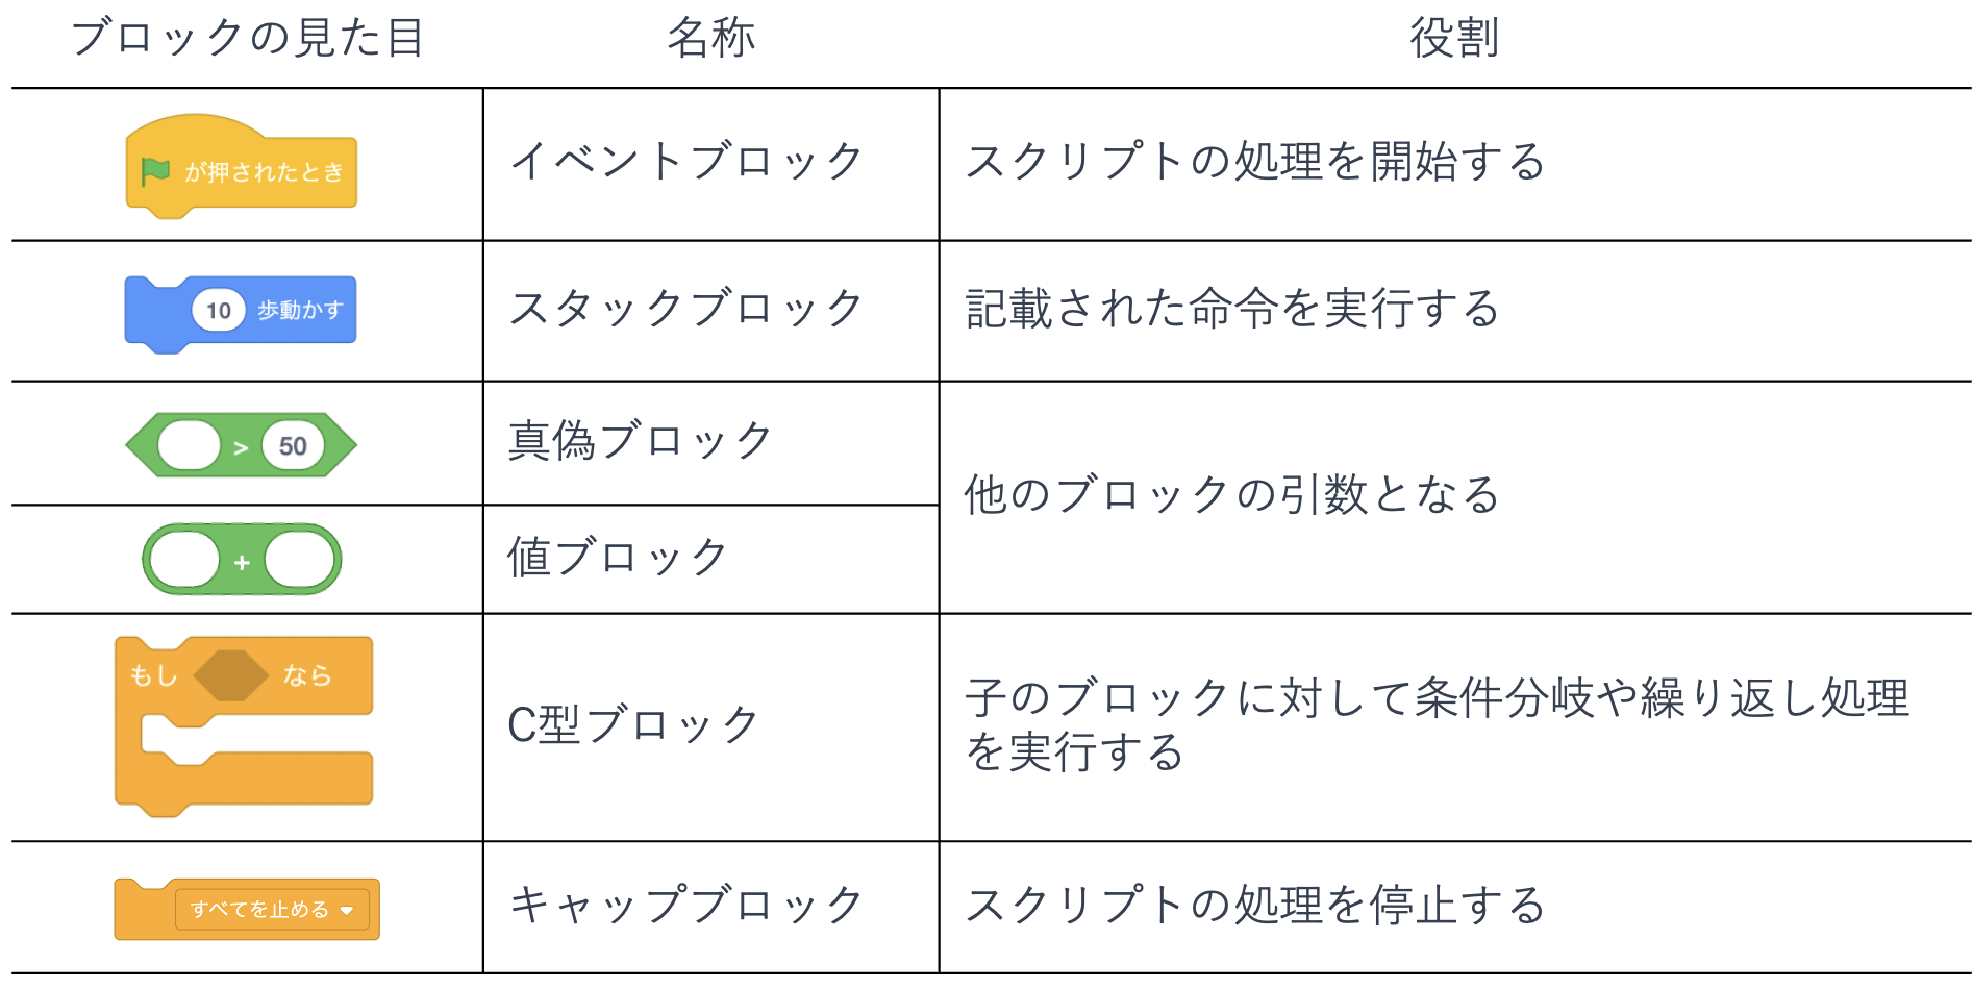
\includegraphics[width=0.9\linewidth]{Okamoto_fig/blocks.pdf}
	\caption{6種類のブロックとその性質}
	\label{fig:blocks}
\end{figure*}

\section{作品解析ツール:Dr.Scratch}
近年のプログラミング学習における学習者の目的の一つとして,コンピュテーショナルシンキング(CT)~\cite{Wing_2006}を身につけることが挙げられる.CTとはプログラミングの問題に対する抽象的な分析や,その問題を解決するための効率的な考え方の総称であり,主に問題を応用可能な一般式にする抽象化,問題を一般式に当てはめて表現する実装,問題を解いて確かめる分析の3手順の反復によって習熟していく.Scratchにおいてもプログラムの命令処理の結果がスプライトの動きとして出力されるため,作品制作のプログラム実装を通してCTを身につけることができる.しかし,ユーザが身につけたCTを把握するには,プログラムの実装内容を解析する必要があるため,プログラミング初学者にとって自身のCTを把握することは困難である.Scratchを用いたプログラミング学習を支援するツールとして,Morenoらはユーザが制作した作品に必要なCTを評価するDr.Scratch~\cite{Moreno_2015}を開発している.Dr.Scratchは,Scratch作品で利用されたブロックやプログラムの構造からCTスキルを計測し,7つの概念(CT7概念:抽象化,並列,論理,動機,フロー制御,ユーザ対話性,データ表現)で結果を出力する.表\ref{tab:analysis_method}に7概念の計測方法を示す.各CT概念は,作品中に使用されたブロックの種類やその数に基づいて,それぞれ0点から3点の4段階の点数によって評価される.また,作品自体はそれぞれのCT概念の点数を合計した0点から21点の22段階(CTスコア)で評価される.特に,CTスキルの区分としてCT習熟度が存在し,0点から7点をBasic,8点から14点をDeveloping,15点から21点をMasterとして3区分で評価している.

図\ref{fig:drscratch}はDr.Scartchによる作品の評価結果を示す.図\ref{fig:drscratch}には作品の制作にフロー制御,ユーザ対話性,データ表現が2点とそれ以外の概念が0点必要であると算出され,CTスコア合計点が6点として習熟度がBasicと評価している.このように,ユーザは制作した作品をDr.Scratchによって各CT概念を0点から3点で評価し,CT概念の合計点に基づき,CTスキルを獲得する.CT概念の一部は,同一概念に関わらず作品内で使用されるブロックの種類によって異なる点数を決定する.例えば.「同期」の概念では,待機ブロックを使用することで1点を獲得することができるが,メッセージブロックを使用してプログラムを停止する機能を実装する場合は2点を獲得する.

本研究ではユーザのCTを明確に捉えるため,過去に制作した作品で使用する各CT概念の0点から3点までを区別して調査する.

\begin{table}[t]
    \caption{Dr.Scratchによる7つのCT概念の評価方法~\cite{Moreno_2015}}\label{tab:analysis_method}
    \vspace{2mm}
    \centering
    \scalebox{0.65}{
        \begin{tabular}{l|c|c|c}
            \hline
            \multicolumn{1}{c|}{CT概念} & 1点 & 2点 & 3点 \\ \hline 
            \hline
            抽象化 & \multicolumn{1}{c|}{2つ以上のスクリプトを使用} & \multicolumn{1}{c|}{定義ブロックを使用} & \multicolumn{1}{c}{クローンブロックを使用} \\ \hline
            並列 & \begin{tabular}{c}緑の旗ブロックを2個以上使用\end{tabular} & \begin{tabular}{c}オブジェクトへのクリック動作により\\2つ以上のスクリプトを同時に\\実行する機能を実装\end{tabular} & \begin{tabular}{c}背景の切り替え,メッセージの受け取り\\など,イベント動作により2つ以上の\\スクリプトを同時に実行する機能を実装\end{tabular} \\ \hline
            論理 & Ifブロックを使用 & If elseブロックを使用 & 論理演算ブロックを使用 \\ \hline
            同期 & 待機ブロックを使用 & \begin{tabular}{c}メッセージを受信すると\\プログラムを停止する機能を実装\end{tabular} & \begin{tabular}{c}指定条件を満たすまで\\プログラムを停止する処理を実装\end{tabular} \\ \hline
            フロー制御 & 2個以上の処理ブロックを連結して使用 & \begin{tabular}{c}指定回数,または回数無制限の\\繰り返しブロックを使用\end{tabular} & 指定条件までの繰り返しブロックを使用 \\ \hline
            ユーザ対話性 & 緑の旗ブロックを使用 & \begin{tabular}{c}ユーザによる入力を伴うブロックを使用\end{tabular} & \begin{tabular}{c}マイクやビデオなど\\インタラクションを伴うブロックを使用\end{tabular} \\ \hline
            データ表現 & \begin{tabular}{c}オブジェクトの大きさや位置等の\\プロパティを編集\end{tabular} & 変数ブロックを使用 & リスト変数ブロックの使用 \\ \hline
        \end{tabular}
    }
\end{table}

\begin{figure*}[t]
	\centering
	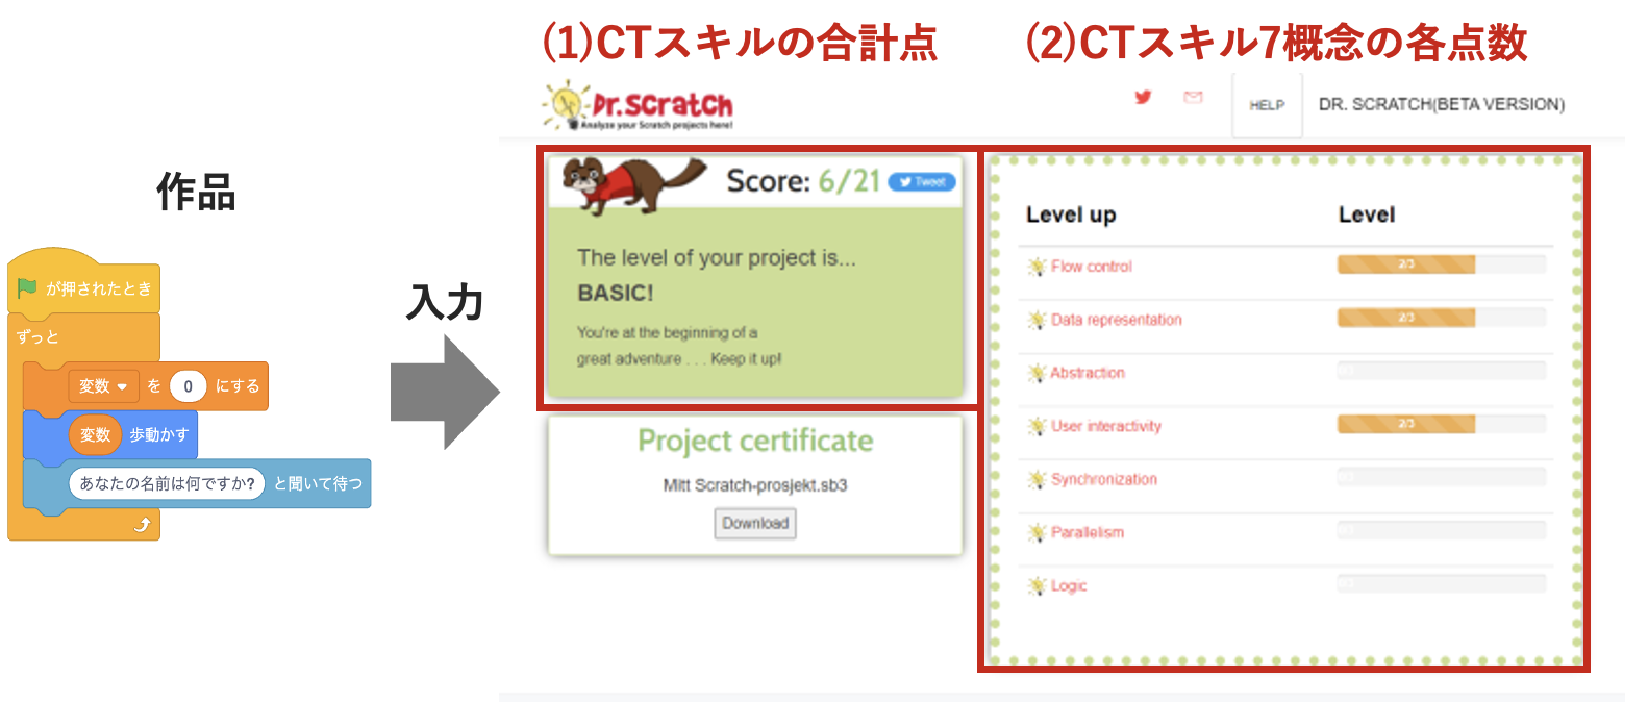
\includegraphics[width=1.0\linewidth]{Okamoto_fig/drscratch.pdf}
	\caption{Dr.Scratchの評価画面と評価方法}
	\label{fig:drscratch}
\end{figure*}

\section{従来研究}
Scratchにおけるユーザのプログラミング能力の成長に関する研究として,Yangら~\cite{Yang_2015}はScratch
で50回以上の作品を制作したユーザ3,852人を対象に,作品制作回数の増加に伴うユーザが使用するブロックの種類数を調査している.その結果,ユーザは作品制作過程を経る毎に作品に使用するブロックの種類が増加し,リミックス(他のユーザの作品を再利用すること)の機能を用いているユーザほどその増加数が大きいことが明らかとなった.

Troianoら~\cite{Troiano_2019}は,13歳から14歳の生徒19人を対象に,それぞれの作品制作過程で作品に使用するCT概念を調査した.その結果,作品制作過程を経るごとに並列,論理,同期の点数が高くなる生徒が多いが,抽象化やデータ表現の点数が高くなる生徒が少ないことを示した.また,生徒が最終的に到達するCTスコアや,点数を伸ばすまでにかかる時間は,制作する作品のジャンル(シューティングゲームやアクションゲーム等)によって異なることを明らかにした.

安東ら~\cite{Ando_2021}はユーザのCTに合わせた作品推薦に向けて,ユーザが過去に制作した作品のCTスキルに基づいてユーザが次にCT習熟度が向上するかを予測する研究を行なった.事前分析としてユーザがScratch上に公開している作品を収集し,各作品で使用されるCT概念をDr.Scratchを用いて計測し,ユーザが特定の習熟度に到達するまでに制作した作品の特徴を分析した.分析結果として,ユーザにとって習熟度DevelopingやMasterに分類されるオリジナル作品の制作は困難であり,ユーザは類似するCTスコアの作品を連続して制作することで習熟度が向上することが示唆された.特に,習熟度Developingのオリジナル作品を制作するまでに,ユーザは連続してBasicやDevelopingの作品を制作することが多く,Masterの作品を制作することは少ないことがわかり,習熟度Masterのオリジナル作品を制作するユーザの数は少なく,Masterの作品を連続して制作することは少ないことがわかった.また,ユーザが過去に使用したCT概念に基づき,ユーザが次に制作する作品が当該習熟度以上の評価を得るかを予測モデルとして,事前分析の結果に基づき,目的変数の異なる2種類のモデルを構築した.

\begin{description}
\item [モデル1:]習熟度がDeveloping以上のオリジナル作品を制作するユーザを予測
\item [モデル2:]習熟度がMasterのオリジナル作品を制作するユーザを予測
\end{description}

説明変数としてはユーザが過去に作品制作で使用した7つのCT概念の0点から3点の獲得有無を用いた.モデルの構築にはランダムフォレストを用いており,事前分析で収集したデータを基に構築,予測を行った.結果としてDevelopingやMasterに到達するユーザと到達しないユーザの間では,過去に使用したCT概念に違いがあることが示唆された.

多くの従来研究では,Scratch上でユーザが制作する作品の特徴,または作品制作過程全体で使用するCT概念を調査しており,一部のCT概念の学習が困難であること,また特定の習熟度に到達するユーザとそうでないユーザ間では獲得したCT概念に違いがあることを明らかにしている.しかし,従来研究ではCT7概念の詳細な獲得過程については明らかになっていない.

安東らは,学習者のCT習熟度の把握を目的として,ScratchユーザのCT習熟度予測を行った.表\ref{tab:same-path}は従来研究\cite{Ando_2021}の対象ユーザのうち,CTパス:ユーザが獲得してきたCT7概念が同じだったユーザのペア数と従来モデルの予測結果が異なるペア数,予測がどちらも外れたペア数を示す.表\ref{tab:same-path}のモデル1では,予測がどちらも外れたペア数が512と多く,予測結果が異なるペア数と予測がどちらも外れたペア数を合わせるとCTパスが同じ全てのペアのうち,約13\%が予測が異なる,あるいは予測が外れていることがわかる.また,表\ref{tab:same-path}のモデル2では予測結果が異なるペア数と予測がどちらも外れたペア数のどちらも数は小さいものの,CTパスが同じ全てのペア数のうち,約30\%を占めていることがわかる.このことから,従来モデルではユーザのCT概念の獲得有無のみを説明変数としているため,ユーザのCT概念獲得過程は考慮されていないことが考えられる.しかし,実際にユーザは習熟度が向上するまでに様々な作品制作過程があることを確認している.

したがって,ユーザのCT7概念の獲得過程に基づいて,当該ユーザが保有するCTの習熟度の特定ができれば,ScratchにおけるユーザのCTスキル獲得状況に合わせた学習の参考となる作品提示等の学習支援の役立てとなると期待する.

\begin{table}
  \caption{同じCTパスを持つユーザのペア数}
  \label{tab:same-path}
  \vspace{2mm}
  \centering
  \begin{tabular}{c|c|c|c}
    \hline
     & 予測結果が異なるペア数 & 予測がどちらも外れたペア数 & 全てのペア数\\
    \hline
    \hline
    モデル1 & 24 & 512 & 4,094 \\
    \hline
    モデル2 & 14 & 5 & 63 \\
    \hline
  \end{tabular}
\end{table}



% \section{動機}
% 近年,プログラミング教育において学習者の成長過程を把握することは重要視されており,関連する研究が多数報告されている.Özgenら\todo{引用:Comparing Students’ Scratch Skills with Their Computational Thinking Skills in Terms of Different Variables}はScratchにおいて学習者がコンピュータの使用期間によってCTスコアが異ならないことを明らかにした.Ruijiaら\todo{引用:How Interest-Driven Content Creation Shapes Opportunities for Informal Learning in Scratch: A Case Study on Novices’ Use of Data Structures}はScratch上で公開されているプログラムを解析し,時間経過によって学習者がプログラムに変数やリストを使う数が増加することが明らかとなった.これらの研究では学習者のCTスキルの成長過程は分析,把握していない.しかし,プログラミング学習の目的はプログラムの実装方法の学習を通してCTを身につけることにあるため,教育者にとって学習者のCTスキルの成長過程を把握することは重要である.従来研究では学習者のCT習熟度の把握を目的として,ScratchユーザのCT習熟度予測を行った.\todo{説明変数一緒で予測違うペアの統計}は従来研究における予測結果のうち,CTパス:ユーザが獲得してきたCT7概念が同じで,予測結果が異なる結果の数を示した表である.また,\todo{説明変数一緒でどっちも外れたやつ}は従来研究における予測結果のうち,CTパスが同じで,予測結果がどちらも外れた結果の数を示している.表1のモデル1では予測結果が異なる割合が多く,表2のモデル1では半分以上が予測結果が外れていることがわかる.このことから,従来モデルではユーザのCTパスは考慮できておらず,精度が落ちてしまっていることが考えられる.

% 本研究では,ScratchユーザのCTスキルの成長過程の把握を目的として,続く\todo{次の章}で設定するリサーチクエスチョンに基づきScratchユーザのCT成長過程の分析を行い,次に学習者がCT習熟度が向上するかの到達予測を行う.本研究により,Scratchにおいてユーザの成長過程に合わせた学習支援の役立てとなることを期待する.


\section{リサーチクエスチョン(RQ)}
本章では目的達成のために設定したRQの動機について説明する.
\subsection{RQ1:CT習熟度が向上したユーザが獲得してきたCT7概念の違いはどの程度か?}
RQ1ではScratch作品の制作過程でCT習熟度が向上したユーザに着目して,各ユーザのCT7概念の獲得過程(CTパス)の特徴量を分析する.本RQではCTパスの特徴量を分析することで,ユーザのCTパスの特徴,ユーザのCT概念の獲得過程に意味があるかを確認する.具体的には,ユーザのCT習熟度が向上する地点までの作品のCT7概念を計測し,CT習熟度が向上するまでに制作した作品数やCTパスの重複数を分析する.また,CTパス中に含まれるCT7概念にも着目し,成長過程によって用いられるCTスキルが異なるかどうかも確認する.詳しい内容については3章で説明する.
\subsection{RQ2:ユーザが獲得してきたCT7概念から次にCT習熟度が向上するかどうかを予測することは可能か?}

RQ2では学習者のCT7概念の獲得過程を考慮した学習支援のため,ユーザのCTスコア獲得過程を説明変数として学習モデルを作成し,ユーザが特定の習熟度に到達するか否かの予測を行う.また,評価の際は従来モデルとの比較を行う.詳しい内容については4章で説明する.


\chapter{RQ1:CT習熟度が向上した多くのユーザが獲得してきたCT7概念の違いはどの程度か?}\label{sec:chapter_3}
\section{概要}
本章では,作品制作の過程でCT習熟度が向上したユーザに焦点を当て,各ユーザが獲得してきたCT7概念の特徴を明らかにする.

従来研究では,ユーザがCT習熟度を向上させる過程でどのようなCTスキルを獲得しているかは詳細に分析されていない.習熟度が向上するまでにユーザが獲得してきたCT7概念(CTパス)の違いを明らかにするために,ユーザの習熟度が向上する地点までの作品におけるCT7概念を計測する.また,CT習熟度が向上するまでに制作した作品の数やCTパスの重複数を基に,作品制作過程とCT概念の特徴をそれぞれ分析する.


\section{データセット}\label{sec:chapter_3-1}
Scratchは2019年1月3日に作品制作に使用可能な命令処理を一部追加,削除,名前の変更をする等,大規模なアップデートを実施しており,このアップデートに伴ってmicro:bitやLEGO MINDSTORMS 等の外部デバイスを用いた学習も行うことができるようになった.従来研究では,ユーザが共通の開発環境で制作した作品を比較するため,バージョン3.0をリリースした2019年1月3日から2020年1月3日までの間に初めて作品公開を行ったユーザを分析対象とし,サービス上に20件以上の作品を公開しているユーザ7,050人が制作した作品141,000件(7,050人×20件)を収集した.本研究ではそれらの作品をDr.ScratchによりCTスコアの計測を行い,失敗しなかった作品を制作したユーザ6,323人が1番目から20番目までに制作した作品126,460件を本分析の対象とする.


\section{分析手法}\label{sec:chapter_3-2}
従来研究~\cite{Ando_2021}ではユーザが一度でも特定の習熟度を満たす作品を制作すれば当該習熟度に到達したと判断しており,リミックス作品による獲得は習熟度到達として認めていない.本研究では,従来研究の設定と同様に,20番目の作品を制作するまでにBasicからDeveloping以上に向上したユーザ(BtoDユーザ)3,125人,DevelopingからMasterに向上したユーザ(DtoMユーザ)1,196人を分析対象とする.また,20番目の作品を制作する過程で,BasicからDevelopingに向上し,さらにDevelopingからMasterに向上するユーザもいるため,BtoDユーザとDtoMユーザの間には重複がある.

本分析では,BtoDユーザとDtoMユーザそれぞれについて,習熟度が向上するまでに獲得したCT7概念の系列(CTパス)を抽出する.リミックス作品も学習の一部とみなし,習熟度向上の過程で制作されたリミックス作品もCTパスに含める.

図\ref{fig:digraph}は2人のBtoDユーザのCTパスの事例を状態遷移図として示す.図中のノードは,制作された作品から測定されたCT7概念のスコア分布を示し,次に制作する作品へのつながりはエッジで表現する.各ノード内のレーダーチャートのラベル記号は,対応するCT7概念に一致し,表\ref{tab:ct-symobol}にその対応関係を示す.各項目はチャートの最外側が3点,最内側が0点とする.図\ref{fig:digraph}のBtoDユーザAは最初に全てのCTスコアが0点の作品を制作し,次にフロー制御,ユーザ対話性,データ表現の概念を1点を獲得した後,ユーザ対話性と論理の概念で2点向上させ,習熟度Developingに到達している.

多くのユーザが経由する作品制作過程の特徴を分析するため,各ユーザがCT習熟度が向上するまでに制作した作品数と,BtoDユーザ,DtoMユーザ毎のエッジの重複数を算出する.例えば,図\ref{fig:digraph}のユーザAは習熟度が向上するまでに制作した作品数が3であり,ユーザBは2である.また,ノード$A_1$とノード$B_1$,ノード$A_2$とノード$B_2$で制作された作品は同じCT概念を用いているため,CTパスが重複している.ユーザの作品制作過程の再現性を確認するため,ユーザのCTパス重複数として,ユーザのCTパスの各エッジの重複数を合計し,エッジ数で割った平均値を用いる.ユーザAとユーザBのみを分析する場合,ユーザAの各エッジの重複数は1,2,2となり,ユーザAのCTパス重複数は$(1 + 2 + 2) / 3 = 1.67$となる.

本分析では,より特徴のあるCTパスを抽出するため,習熟度を向上させる際に制作した作品のCT概念の重複数が多いユーザに着目する.また,ユーザが習熟度向上までにかかる時間による違いも明らかにするため,習熟度向上までに制作した作品数毎のCTパス(代表CTパス)を抽出する.代表CTパスは習熟度向上までに制作した作品数毎に取得したCTパスに対し,以下の操作を行なって抽出する.
\begin{enumerate}
    \item 習熟度向上までに制作した作品数毎に各エッジの重複数を算出する.
    \item 習熟度向上の際に作成した作品から最大のエッジの重複数を持つノードに移る.
    \item 現在のノードの直前にある最大のエッジの重複数を持つノードを確認する.
    \item 最大のエッジの重複数を持つノードが一つしか存在しなかった場合そのノードに移り,3の操作を行う.複数ある場合は5の操作を行う.現在のノードが初期ノードである場合,6の操作を行う.
    \item ユーザ全体のCTパスから各エッジの重複数(重要度)を算出し,4で特定した複数のエッジの中から,重要度が最も高いエッジの重複数を持つノードに移り,3の操作を行う.現在のノードが初期ノードである場合,6の操作を行う.
    \item 現在のノードまでに辿ってきたパスを代表CTパスとして抽出する.
\end{enumerate}



\begin{figure*}[t]
	\centering
	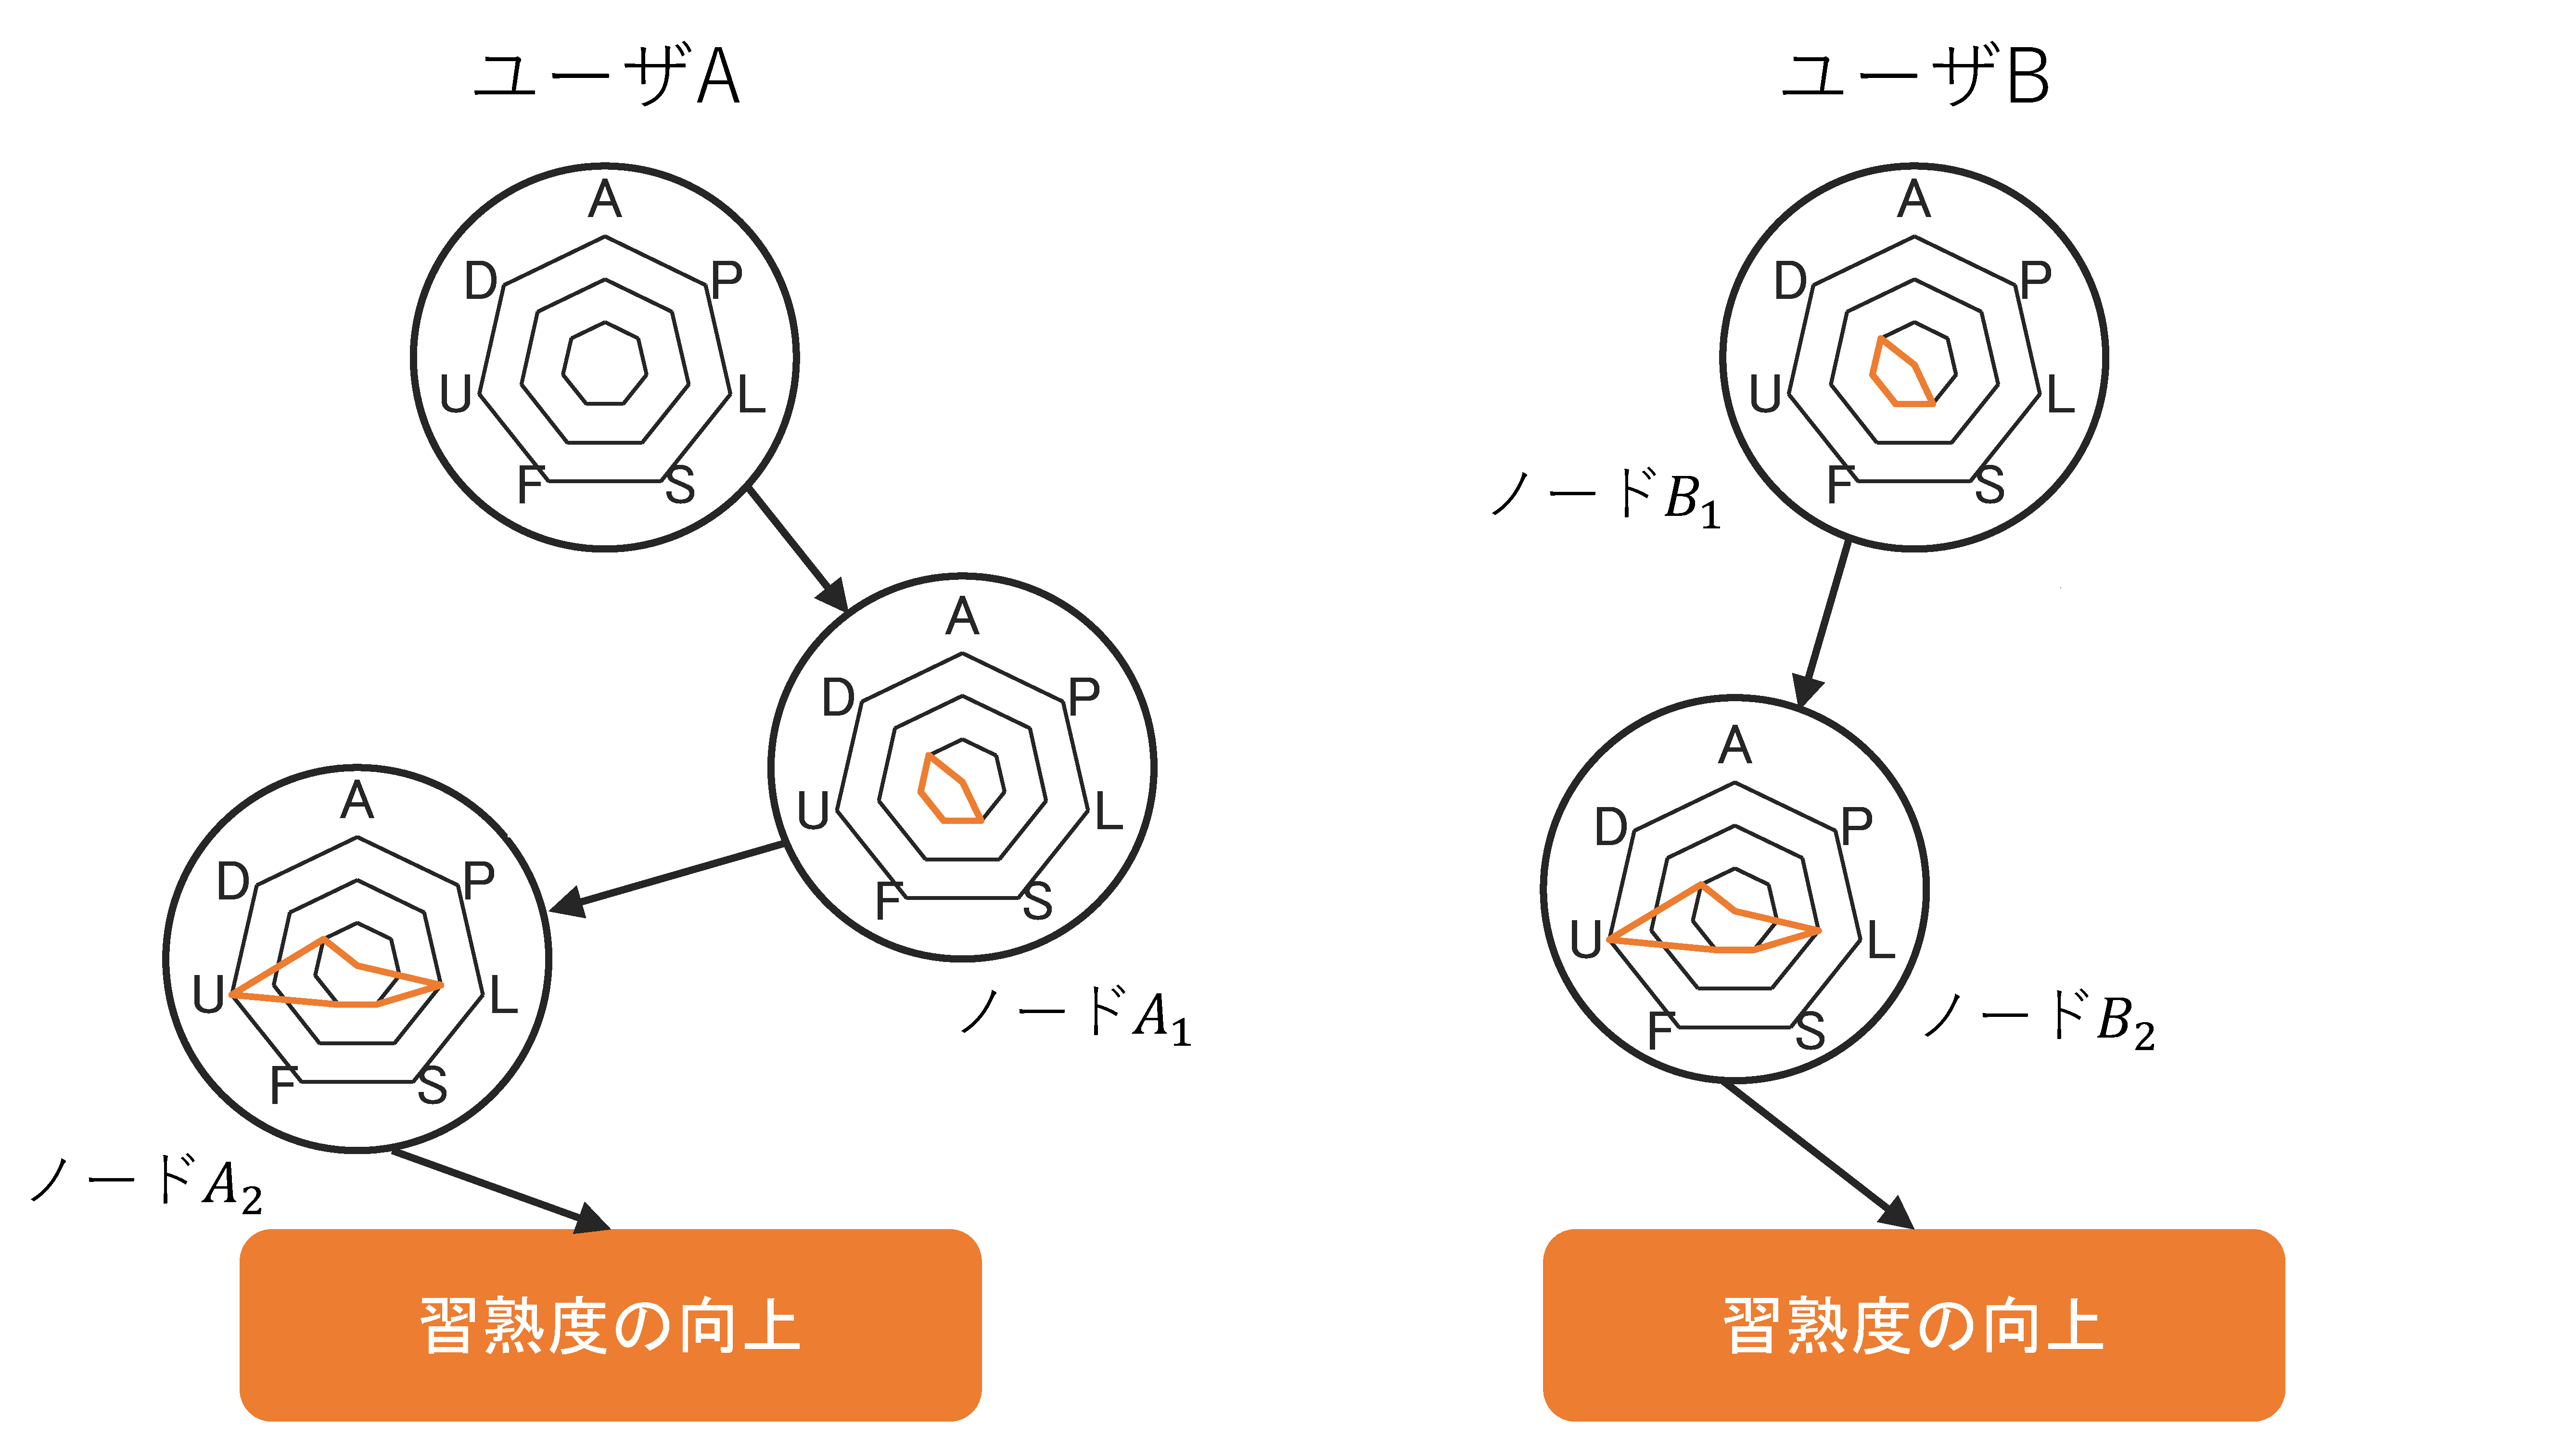
\includegraphics[width=1.0\linewidth]{Okamoto_fig/digraph.pdf}
	\caption{BtoDユーザ二人のCTパスを示した状態遷移図}
	\label{fig:digraph}
\end{figure*}

\begin{table}
  \caption{記号とCT7概念の対応表}
  \label{tab:ct-symobol}
  \vspace{2mm}
  \centering
  \begin{tabular}{c|c}
    \hline
    記号 & CT7概念\\
    \hline
    \hline
    A & 抽象化 \\
    \hline
    P & 並列 \\
    \hline
    S & 同期 \\
    \hline
    L & 論理 \\
    \hline
    F & フロー制御 \\
    \hline
    U & ユーザ対話性 \\
    \hline
    D & データ表現 \\
    \hline
  \end{tabular}
\end{table}




\section{分析結果}\label{sec:3-analysis}
\subsection{作品制作過程の特徴量分析}\label{subsec:path-analysis}
図\ref{fig:dupli-mean}は各習熟度レベルへ向上したユーザのCTパスの重複数を示す箱ひげ図である.BtoDユーザのCTパスの重複数に関して,中央値が10.5,平均値が35.8であることから,BasicからDeveloping以上のレベルに習熟度が到達するユーザは,再現性のあるCTパスをたどって習熟度を向上させていることがわかる.一方,DtoMユーザのCTパスの重複数においては,中央値が1.0,平均値が2.4となっており,DevelopingからMasterレベルに習熟度を向上させるユーザは,より多様なCTパスを経由して習熟度を向上させていることが示されている.BtoDユーザとDtoMユーザ間でMann-Whitney U検定\cite{Mann1947OnAT}を適用した結果,統計的に有意差(p値$<$0.05)が確認されたことから,BtoDユーザとDtoMユーザが異なるCTパスを辿って習熟度を向上させていることを示している.

また,図\ref{fig:path-length}は各習熟度レベルに向上するまでにユーザが制作する作品数の分布を示す箱ひげ図である.BtoDユーザが習熟度を向上させるまでに制作する作品数の中央値は6.0,平均値は7.2であり,DtoMユーザのそれは中央値が10.0,平均値が9.6であった.BtoDユーザとDtoMユーザ間でMann-Whitney U検定を実施したところ,統計的に有意な差(p値$<$0.05)が見られたことから,習熟度を向上させる過程で必要とする作品数にはグループ間で差があり,BtoDユーザはDtoMユーザに比べてより短期間で特定の習熟度に到達している.

\begin{figure*}[t]
	\centering
	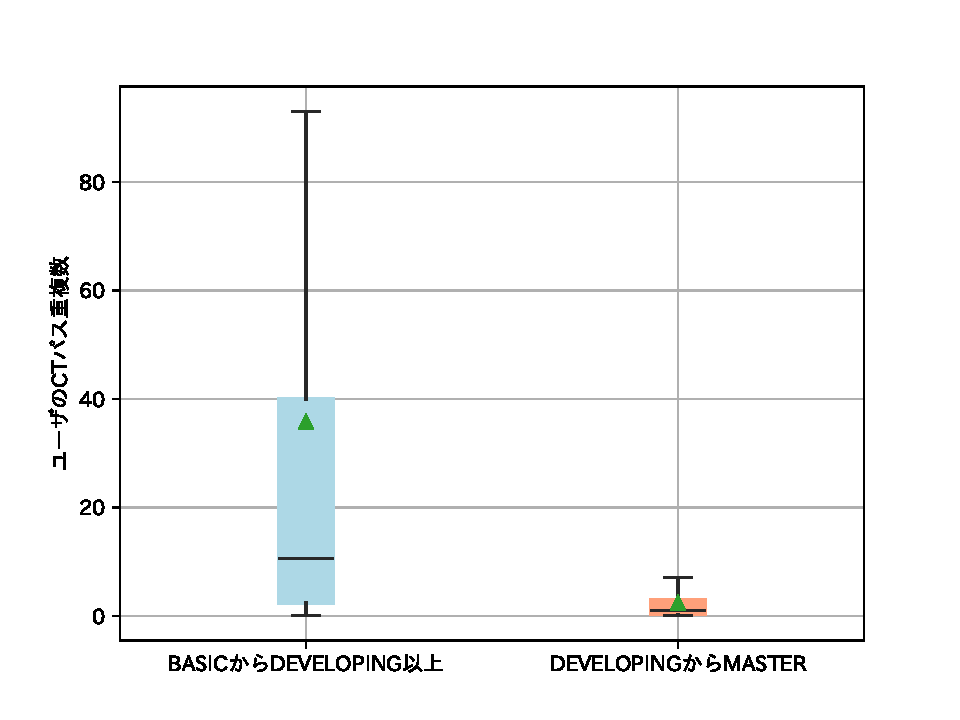
\includegraphics[width=0.8\linewidth]{Okamoto_fig/dupli-all.pdf}
        \vspace{-5mm}
	\caption{各習熟度に到達したユーザのCTパス重複数平均値の分布}
	\label{fig:dupli-mean}
\end{figure*}

\begin{figure*}[t]
	\centering
	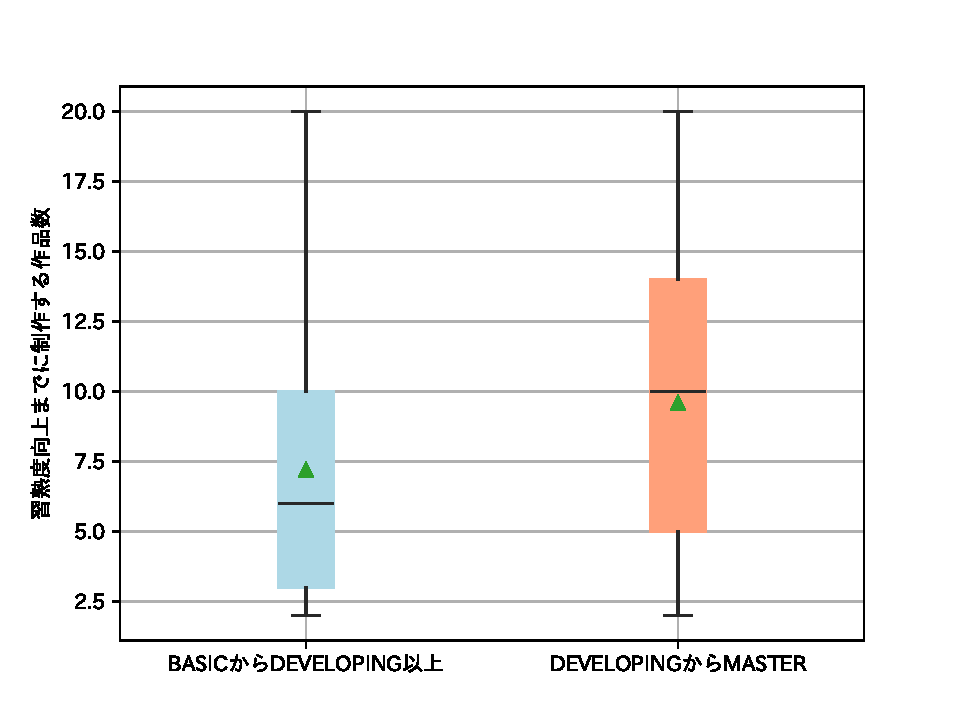
\includegraphics[width=0.8\linewidth]{Okamoto_fig/path-length.pdf}
        \vspace{-5mm}
	\caption{各習熟度に到達したユーザが習熟度向上までに制作する作品数の分布}
	\label{fig:path-length}
\end{figure*}

\subsection{CT獲得過程の分析}\label{subsec:ct-analysis}

表\ref{tab:ranking-btod}にBtoDユーザの中で,習熟度を向上させる際に制作した作品のCT概念の重複数が上位10件にランクされたユーザを示す.CT概念に用いている記号は\ref{sec:chapter_3-2}節で用いた表\ref{tab:ct-symobol}と対応している.データセットから抽出した全BtoDユーザ3,125人の中で,表\ref{tab:ranking-btod}に示す上位10件のCT概念を使用する作品制作したユーザ数は1,209人(約39\%)である.この1,209人の各CT概念において,全ユーザが抽象化で1点を獲得しており,8位を除く全てでデータ表現のスキルを1点獲得している.つまり,多くのBtoDユーザが最終的に抽象化とデータ表現のスキルを獲得していることを示している.

\begin{table}[]
\caption{BtoDユーザが習熟度向上の際に制作する作品のCTスコア重複数の上位10件}
  \label{tab:ranking-btod}
  \vspace{2mm}
  \centering
\begin{tabular}{c|c|cccccccc}
\hline
\multirow{2}{*}{順位} & \multirow{2}{*}{ユーザ数} & \multicolumn{8}{c}{CTスコア}                                                                                               \\ \cline{3-10} 
                    &                      & \multicolumn{1}{c|}{抽象化}  & \multicolumn{1}{c|}{並列} & \multicolumn{1}{c|}{論理} & \multicolumn{1}{c|}{同期} & \multicolumn{1}{c|}{フロー制御} & \multicolumn{1}{c|}{ユーザ対話性} & \multicolumn{1}{c|}{データ表現} & 合計 \\ \hline
                    \hline
1                   & 291                  & \multicolumn{1}{c|}{1} & \multicolumn{1}{c|}{2} & \multicolumn{1}{c|}{0} & \multicolumn{1}{c|}{1} & \multicolumn{1}{c|}{2} & \multicolumn{1}{c|}{2} & \multicolumn{1}{c|}{1} & 9  \\ \hline
2                   & 227                  & \multicolumn{1}{c|}{1} & \multicolumn{1}{c|}{2} & \multicolumn{1}{c|}{0} & \multicolumn{1}{c|}{0} & \multicolumn{1}{c|}{2} & \multicolumn{1}{c|}{2} & \multicolumn{1}{c|}{1} & 8  \\ \hline
3                   & 154                  & \multicolumn{1}{c|}{1} & \multicolumn{1}{c|}{1} & \multicolumn{1}{c|}{0} & \multicolumn{1}{c|}{1} & \multicolumn{1}{c|}{2} & \multicolumn{1}{c|}{2} & \multicolumn{1}{c|}{1} & 8  \\ \hline
4                   & 118                  & \multicolumn{1}{c|}{1} & \multicolumn{1}{c|}{2} & \multicolumn{1}{c|}{0} & \multicolumn{1}{c|}{1} & \multicolumn{1}{c|}{1} & \multicolumn{1}{c|}{2} & \multicolumn{1}{c|}{1} & 8  \\ \hline
5                   & 107                  & \multicolumn{1}{c|}{1} & \multicolumn{1}{c|}{1} & \multicolumn{1}{c|}{1} & \multicolumn{1}{c|}{0} & \multicolumn{1}{c|}{2} & \multicolumn{1}{c|}{2} & \multicolumn{1}{c|}{1} & 8  \\ \hline
6                   & 82                   & \multicolumn{1}{c|}{1} & \multicolumn{1}{c|}{1} & \multicolumn{1}{c|}{0} & \multicolumn{1}{c|}{2} & \multicolumn{1}{c|}{2} & \multicolumn{1}{c|}{1} & \multicolumn{1}{c|}{1} & 8  \\ \hline
7                   & 67                   & \multicolumn{1}{c|}{1} & \multicolumn{1}{c|}{3} & \multicolumn{1}{c|}{0} & \multicolumn{1}{c|}{2} & \multicolumn{1}{c|}{2} & \multicolumn{1}{c|}{1} & \multicolumn{1}{c|}{1} & 10 \\ \hline
8                   & 60                   & \multicolumn{1}{c|}{1} & \multicolumn{1}{c|}{1} & \multicolumn{1}{c|}{1} & \multicolumn{1}{c|}{0} & \multicolumn{1}{c|}{2} & \multicolumn{1}{c|}{2} & \multicolumn{1}{c|}{2} & 9  \\ \hline
9                   & 52                   & \multicolumn{1}{c|}{1} & \multicolumn{1}{c|}{3} & \multicolumn{1}{c|}{0} & \multicolumn{1}{c|}{3} & \multicolumn{1}{c|}{1} & \multicolumn{1}{c|}{1} & \multicolumn{1}{c|}{1} & 10 \\ \hline
10                  & 51                   & \multicolumn{1}{c|}{1} & \multicolumn{1}{c|}{3} & \multicolumn{1}{c|}{0} & \multicolumn{1}{c|}{2} & \multicolumn{1}{c|}{1} & \multicolumn{1}{c|}{1} & \multicolumn{1}{c|}{1} & 9 \\ \hline
\end{tabular}
\end{table}

表\ref{tab:ranking-dtom}にDtoMユーザの中で,習熟度を向上させる際に制作した作品のCT概念の重複数が上位10件にランクされたユーザを示す.CT概念に用いている記号は\ref{sec:chapter_3-2}節で用いた表\ref{tab:ct-symobol}と対応している.データセットから抽出した全DtoMユーザ1,196人の中で,表\ref{tab:ranking-dtom}に示す上位10件のCT概念を使用する作品制作したユーザ数は523人(約44\%)であった.この523人の各CT概念において,全ユーザがユーザ対話性とデータ表現のスキルで2点を獲得しており,10位を除く全てで並列処理のスキルを3点獲得している.これは,多くのDtoMユーザが最終的にユーザ対話性,データ表現,並列処理のスキルを獲得していることを示している.

\begin{table}[]
\caption{DtoMユーザが習熟度向上の際に制作する作品のCTスコア重複数の上位10件}
  \label{tab:ranking-dtom}
  \vspace{2mm}
  \centering
\begin{tabular}{c|c|cccccccc}
\hline
\multirow{2}{*}{順位} & \multirow{2}{*}{ユーザ数} & \multicolumn{8}{c}{CTスコア}                                                                                                                                                         \\ \cline{3-10} 
                    &                      & \multicolumn{1}{c|}{抽象化} & \multicolumn{1}{c|}{並列} & \multicolumn{1}{c|}{論理} & \multicolumn{1}{c|}{同期} & \multicolumn{1}{c|}{フロー制御} & \multicolumn{1}{c|}{ユーザ対話性} & \multicolumn{1}{c|}{データ制御} & 合計 \\ \hline \hline
1                   & 112                  & \multicolumn{1}{c|}{3} & \multicolumn{1}{c|}{3} & \multicolumn{1}{c|}{3} & \multicolumn{1}{c|}{3} & \multicolumn{1}{c|}{3} & \multicolumn{1}{c|}{2} & \multicolumn{1}{c|}{2} & 19  \\ \hline
2                   & 84                  & \multicolumn{1}{c|}{1} & \multicolumn{1}{c|}{3} & \multicolumn{1}{c|}{3} & \multicolumn{1}{c|}{2} & \multicolumn{1}{c|}{2} & \multicolumn{1}{c|}{2} & \multicolumn{1}{c|}{2} & 15  \\ \hline
3                   & 74                  & \multicolumn{1}{c|}{1} & \multicolumn{1}{c|}{3} & \multicolumn{1}{c|}{3} & \multicolumn{1}{c|}{3} & \multicolumn{1}{c|}{2} & \multicolumn{1}{c|}{2} & \multicolumn{1}{c|}{2} & 16  \\ \hline
4                   & 56                  & \multicolumn{1}{c|}{1} & \multicolumn{1}{c|}{3} & \multicolumn{1}{c|}{3} & \multicolumn{1}{c|}{3} & \multicolumn{1}{c|}{3} & \multicolumn{1}{c|}{2} & \multicolumn{1}{c|}{2} & 17  \\ \hline
5                   & 55                  & \multicolumn{1}{c|}{1} & \multicolumn{1}{c|}{3} & \multicolumn{1}{c|}{2} & \multicolumn{1}{c|}{3} & \multicolumn{1}{c|}{2} & \multicolumn{1}{c|}{2} & \multicolumn{1}{c|}{2} & 15  \\ \hline
6                   & 31                   & \multicolumn{1}{c|}{1} & \multicolumn{1}{c|}{3} & \multicolumn{1}{c|}{2} & \multicolumn{1}{c|}{2} & \multicolumn{1}{c|}{3} & \multicolumn{1}{c|}{2} & \multicolumn{1}{c|}{3} & 16  \\ \hline
7                   & 29                   & \multicolumn{1}{c|}{1} & \multicolumn{1}{c|}{3} & \multicolumn{1}{c|}{1} & \multicolumn{1}{c|}{3} & \multicolumn{1}{c|}{3} & \multicolumn{1}{c|}{2} & \multicolumn{1}{c|}{2} & 15 \\ \hline
8                   & 28                   & \multicolumn{1}{c|}{1} & \multicolumn{1}{c|}{3} & \multicolumn{1}{c|}{3} & \multicolumn{1}{c|}{2} & \multicolumn{1}{c|}{3} & \multicolumn{1}{c|}{2} & \multicolumn{1}{c|}{2} & 16  \\ \hline
9                   & 27                   & \multicolumn{1}{c|}{3} & \multicolumn{1}{c|}{3} & \multicolumn{1}{c|}{3} & \multicolumn{1}{c|}{2} & \multicolumn{1}{c|}{3} & \multicolumn{1}{c|}{2} & \multicolumn{1}{c|}{2} & 18 \\ \hline
10                  & 27                   & \multicolumn{1}{c|}{3} & \multicolumn{1}{c|}{1} & \multicolumn{1}{c|}{3} & \multicolumn{1}{c|}{2} & \multicolumn{1}{c|}{3} & \multicolumn{1}{c|}{2} & \multicolumn{1}{c|}{2} & 16  \\ \hline
\end{tabular}
\end{table}

\subsubsection*{BtoDユーザの分析}

全BtoDユーザの中から表\ref{tab:ranking-btod}で1位であったユーザ291人を抽出し,習熟度向上までに制作した作品数毎の代表CTパスを抽出した結果を表\ref{tab:split-ct-btod}に示す.表\ref{tab:split-ct-btod}の代表CTパスは記号の羅列として表現されており,頻繁に利用される記号とCTスキルの対応表は表\ref{tab:dict-btod}に示す.例えば,作品数2の代表CTパスがBBであるため,この代表CTパスを通るユーザは抽象化,並列,同期,ユーザ対話性,データ表現で1点,フロー制御で2点を2作品連続で獲得したのち,Developingに到達する作品を制作している.

代表CTパスの中でも,特にBは作品制作数を跨いで8回出現している.これは代表CTパス中に含まれるCTスキルの中で最多の出現回数であり,BのCTスキル,つまり抽象化,並列,同期,ユーザ対話性,データ表現のスキルを1点,フロー制御のスキルを2点を獲得することがDevelopingへの向上につながることが示唆される.

表\ref{tab:split-ct-btod}の作品数2,3,7,8,10,11,12,13,15,18の代表CTパスでは,同じCT概念の作品を複数回連続して制作している.これは,ユーザが同じCT概念を連続で利用することで,習熟度の向上につながることを示唆している.作品数が10以下ではB,F,Jの点数を連続して獲得している一方で,作品数11以上ではN,L,Qを連続して獲得している.B,F,Jには共通してフロー制御が2点,ユーザ対話性とデータ表現が1点含まれる一方,N,L,Qには共通してフロー制御,ユーザ対話性,データ表現が1点ずつ含まれている.このことから,制作する作品数が異なっても,作品制作過程で獲得するCT概念は同じだが,点数が低い方が習熟度の向上に時間がかかることが示唆される.

また,作品数14,16,17の代表CTパスでは,部分的に同じCT概念を繰り返し獲得することで習熟度を向上させている.例えば,作品数14の代表CTパスでは,NBSのCT概念を4回とNBのCT概念を1回獲得したのちに習熟度を向上させている.繰り返して獲得しているCT概念のセットはNBS,UOQV,CYAである.NBSは共通してフロー制御,ユーザ対話性,データ表現を1点ずつ獲得しているセットである.UOQVは途中に二度Master以上のCTスコアを持つ作品をリミックスしている.CYAは4点以下の作品のみを制作し,途中には0点の作品も制作している.このことから,部分的に同じCT概念を繰り返し獲得するユーザのCTパスは,制作する作品数によってその特徴が異なることが示唆される.


\begin{table}[h]
  \begin{minipage}[t]{0.45\linewidth} % 0.5\linewidthはページ幅の半分に相当
    \centering
    \caption{対象BtoDユーザが習熟度向上までに制作した作品数毎の代表CTパス}
    \label{tab:split-ct-btod}
    \vspace{2mm}
  \begin{tabular}{c|l}
    \hline
    作品数 & 代表CTパス\\
    \hline
    \hline
    1 & A \\
    \hline
    2 & BB \\
    \hline
    3 & BBB \\
    \hline
    4 & ACDE \\
    \hline
    5 & FGHFI \\
    \hline
    6 & JBKLJM \\
    \hline
    7 & FFFFFFF  \\
    \hline
    8 & JJJJJJJM \\
    \hline
    9 & NNNHBKHJM \\
    \hline
    10 & BBBBBBBBBO \\
    \hline
    11 & NNNNNNNNPBI \\
    \hline
    12 & NNNNNNNNNNNN \\
    \hline
    13 & LLLLLLLLLLLQR \\
    \hline
    14 & NBSNBSNBSNBSNB \\
    \hline
    15 & QQQQQQQQQQQQQQT \\
    \hline
    16 & UOQVWUOQVWUOQVXB \\
    \hline
    17 & CYACYACYACYACYACZ \\
    \hline
    18 & NNNNNNNNNNNNNNNNNN \\
    \hline
  \end{tabular}
  \end{minipage}%
  \begin{minipage}[t]{0.55\linewidth}
    \centering
    \caption{代表CTパスの記号とCT概念の対応表}
    \label{tab:dict-btod}
    \vspace{8mm}
      \begin{tabular}{c|c|cccccccc}
\hline
\multirow{2}{*}{記号} & \multicolumn{1}{l|}{\multirow{2}{*}{\small{リミックス}}} & \multicolumn{8}{c}{CTスコア}                                                                                                                                                         \\ \cline{3-10} 
                    & \multicolumn{1}{l|}{}                       & \multicolumn{1}{c|}{A} & \multicolumn{1}{c|}{P} & \multicolumn{1}{c|}{L} & \multicolumn{1}{c|}{S} & \multicolumn{1}{c|}{F} & \multicolumn{1}{c|}{U} & \multicolumn{1}{c|}{D} & 合計 \\ \hline \hline
A                   & 0                                           & \multicolumn{1}{c|}{0} & \multicolumn{1}{c|}{0} & \multicolumn{1}{c|}{0} & \multicolumn{1}{c|}{0} & \multicolumn{1}{c|}{1} & \multicolumn{1}{c|}{1} & \multicolumn{1}{c|}{1} & 3  \\ \hline
B                   & 0                                           & \multicolumn{1}{c|}{1} & \multicolumn{1}{c|}{1} & \multicolumn{1}{c|}{0} & \multicolumn{1}{c|}{1} & \multicolumn{1}{c|}{2} & \multicolumn{1}{c|}{1} & \multicolumn{1}{c|}{1} & 7  \\ \hline
C                   & 0                                           & \multicolumn{1}{c|}{0} & \multicolumn{1}{c|}{0} & \multicolumn{1}{c|}{0} & \multicolumn{1}{c|}{0} & \multicolumn{1}{c|}{0} & \multicolumn{1}{c|}{0} & \multicolumn{1}{c|}{0} & 0  \\ \hline
F                   & 0                                           & \multicolumn{1}{c|}{1} & \multicolumn{1}{c|}{1} & \multicolumn{1}{c|}{0} & \multicolumn{1}{c|}{0} & \multicolumn{1}{c|}{2} & \multicolumn{1}{c|}{1} & \multicolumn{1}{c|}{1} & 6  \\ \hline
J                   & 0                                           & \multicolumn{1}{c|}{0} & \multicolumn{1}{c|}{0} & \multicolumn{1}{c|}{0} & \multicolumn{1}{c|}{0} & \multicolumn{1}{c|}{2} & \multicolumn{1}{c|}{2} & \multicolumn{1}{c|}{1} & 5  \\ \hline
L                   & 0                                           & \multicolumn{1}{c|}{0} & \multicolumn{1}{c|}{0} & \multicolumn{1}{c|}{0} & \multicolumn{1}{c|}{1} & \multicolumn{1}{c|}{1} & \multicolumn{1}{c|}{2} & \multicolumn{1}{c|}{1} & 5  \\ \hline
N                   & 0                                           & \multicolumn{1}{c|}{0} & \multicolumn{1}{c|}{0} & \multicolumn{1}{c|}{0} & \multicolumn{1}{c|}{0} & \multicolumn{1}{c|}{2} & \multicolumn{1}{c|}{1} & \multicolumn{1}{c|}{1} & 4  \\ \hline
O                   & 0                                           & \multicolumn{1}{c|}{1} & \multicolumn{1}{c|}{1} & \multicolumn{1}{c|}{0} & \multicolumn{1}{c|}{1} & \multicolumn{1}{c|}{1} & \multicolumn{1}{c|}{1} & \multicolumn{1}{c|}{1} & 6  \\ \hline
Q                   & 0                                           & \multicolumn{1}{c|}{1} & \multicolumn{1}{c|}{0} & \multicolumn{1}{c|}{0} & \multicolumn{1}{c|}{0} & \multicolumn{1}{c|}{1} & \multicolumn{1}{c|}{2} & \multicolumn{1}{c|}{1} & 5  \\ \hline
S                   & 0                                           & \multicolumn{1}{c|}{1} & \multicolumn{1}{c|}{0} & \multicolumn{1}{c|}{0} & \multicolumn{1}{c|}{1} & \multicolumn{1}{c|}{1} & \multicolumn{1}{c|}{2} & \multicolumn{1}{c|}{1} & 6  \\ \hline
U                   & 1                                           & \multicolumn{1}{c|}{3} & \multicolumn{1}{c|}{3} & \multicolumn{1}{c|}{3} & \multicolumn{1}{c|}{3} & \multicolumn{1}{c|}{3} & \multicolumn{1}{c|}{2} & \multicolumn{1}{c|}{3} & 20 \\ \hline
V                   & 1                                           & \multicolumn{1}{c|}{2} & \multicolumn{1}{c|}{3} & \multicolumn{1}{c|}{2} & \multicolumn{1}{c|}{3} & \multicolumn{1}{c|}{3} & \multicolumn{1}{c|}{1} & \multicolumn{1}{c|}{2} & 16 \\ \hline
W                   & 1                                           & \multicolumn{1}{c|}{1} & \multicolumn{1}{c|}{3} & \multicolumn{1}{c|}{0} & \multicolumn{1}{c|}{2} & \multicolumn{1}{c|}{2} & \multicolumn{1}{c|}{1} & \multicolumn{1}{c|}{2} & 11 \\ \hline
Y                   & 0                                           & \multicolumn{1}{c|}{0} & \multicolumn{1}{c|}{0} & \multicolumn{1}{c|}{0} & \multicolumn{1}{c|}{1} & \multicolumn{1}{c|}{1} & \multicolumn{1}{c|}{1} & \multicolumn{1}{c|}{1} & 4  \\ \hline
\end{tabular}
  \end{minipage}
\end{table}

\subsubsection*{DtoMユーザの分析}

全DtoMユーザの中から表\ref{tab:ranking-dtom}で1位であったユーザ112人を抽出し,習熟度向上までに制作した作品毎の代表CTパスを抽出した結果を表\ref{tab:split-ct-dtom}に示す.表\ref{tab:ranking-dtom}の代表CTパスは記号の羅列として表現されており,一度しか用いられないCTスキルは-を使って抽象化されている.頻繁に利用される記号とCTスキルの対応表は表\ref{tab:dict-btod}に示す.表\ref{tab:dict-dtom}のCT概念に用いている記号は\ref{sec:chapter_3-2}で用いた表\ref{tab:ct-symobol}と対応している.また,図\ref{fig:digraph-dtom}はDtoMユーザの代表CTパスを可視化した状態遷移図であり,最下部のノードに習熟度向上時に制作した作品,それ以外のノードには表\ref{tab:split-ct-dtom}と対応する記号を示す.

表\ref{tab:split-ct-dtom}の制作作品数が10以下のユーザは,BtoDユーザと異なり,多様なCTパスを辿ってMasterに到達している.しかし,これらのCTパスでは共通して抽象化,並列,フロー制御,データ表現をそれぞれ1点ずつ獲得していることが確認されるため,制作作品数の少ないDevelopingユーザはこれらのスキルを身につけることでMasterに向上することが示唆される.
表\ref{tab:split-ct-dtom}と図\ref{fig:digraph-dtom}作品数が11以上のユーザは作品数16と18を除いた全てのCTパスでM,c,d,Q,f,g,OのCTスキルを獲得していることが確認できる.M,c,d,Q,f,g,OのパスはCTスコアの平均値が約8点と低く,各作品によって獲得しているCT概念も異なることから,ユーザは一つの作品で複数のスキルを身につけるわけではなく,時間をかけて作品毎に各CT概念のスキルを獲得してMasterに成長していることが示唆される.QはCTスコアが0点の作品であるが,作品制作数の多いユーザではほとんど獲得していることから,0点のオリジナル作品を制作することの学習効果の可能性も示唆される.また,最後は必ずリミックス作品であるOを獲得しており,リミックスによるMasterへの学習効果も示唆された.

\begin{table}[h]
  \begin{minipage}[t]{0.45\linewidth} % 0.5\linewidthはページ幅の半分に相当
    \centering
    \caption{習熟度向上までに制作した作品数毎の代表CTパス}
    \label{tab:split-ct-dtom}
    \vspace{2mm}
  \begin{tabular}{c|l}
    \hline
    作品数 & 代表CTパス\\
    \hline
    \hline
    1 & A \\
    \hline
    2 & BB \\
    \hline
    3 & CDE \\
    \hline
    4 & FFGH \\
    \hline
    5 & IJKLK \\
    \hline
    6 & MNOPQR \\
    \hline
    7 & SSTUVWX  \\
    \hline
    8 & YZZaaaZ - \\
    \hline
    9 & - - - - - QQbb \\
    \hline
    10 & JJ - b - bbbbb \\
    \hline
    11 & McdeQfg - hiO \\
    \hline
    12 & McdjeQfgkhiO \\
    \hline
    13 & McdjeQcfgbZiO \\
    \hline
    14 & McdjeQfg - - k - iO \\
    \hline
    15 & Mcdj - - Qfg - - khNO \\
    \hline
    16 & - - - - c - - - - - - - KOP \\
    \hline
    17 & Mcd - TQQfgkh - - NOPO \\
    \hline
    18 & XX - Xccc - cZHR - cZHXc  \\
    \hline
  \end{tabular}
  \end{minipage}%
  \begin{minipage}[t]{0.55\linewidth}
    \centering
    \caption{代表CTパスの記号とCT概念の対応表}
    \label{tab:dict-dtom}
    \vspace{8mm}
      \begin{tabular}{c|c|cccccccc}
\hline
\multirow{2}{*}{記号} & \multicolumn{1}{l|}{\multirow{2}{*}{\small{リミックス}}} & \multicolumn{8}{c}{CTスコア}                                                                                                                                                         \\ \cline{3-10} 
                    & \multicolumn{1}{l|}{}                       & \multicolumn{1}{c|}{A} & \multicolumn{1}{c|}{P} & \multicolumn{1}{c|}{L} & \multicolumn{1}{c|}{S} & \multicolumn{1}{c|}{F} & \multicolumn{1}{c|}{U} & \multicolumn{1}{c|}{D} & 合計 \\ \hline \hline
B                   & 0                                           & \multicolumn{1}{c|}{3} & \multicolumn{1}{c|}{1} & \multicolumn{1}{c|}{1} & \multicolumn{1}{c|}{2} & \multicolumn{1}{c|}{2} & \multicolumn{1}{c|}{2} & \multicolumn{1}{c|}{2} & 13  \\ \hline
M                   & 0                                           & \multicolumn{1}{c|}{1} & \multicolumn{1}{c|}{1} & \multicolumn{1}{c|}{0} & \multicolumn{1}{c|}{0} & \multicolumn{1}{c|}{3} & \multicolumn{1}{c|}{1} & \multicolumn{1}{c|}{2} & 9  \\ \hline
O                   & 1                                           & \multicolumn{1}{c|}{2} & \multicolumn{1}{c|}{0} & \multicolumn{1}{c|}{3} & \multicolumn{1}{c|}{0} & \multicolumn{1}{c|}{3} & \multicolumn{1}{c|}{2} & \multicolumn{1}{c|}{2} & 12  \\ \hline
Q                   & 0                                           & \multicolumn{1}{c|}{0} & \multicolumn{1}{c|}{0} & \multicolumn{1}{c|}{0} & \multicolumn{1}{c|}{0} & \multicolumn{1}{c|}{0} & \multicolumn{1}{c|}{0} & \multicolumn{1}{c|}{0} & 0  \\ \hline
X                   & 0                                           & \multicolumn{1}{c|}{1} & \multicolumn{1}{c|}{3} & \multicolumn{1}{c|}{0} & \multicolumn{1}{c|}{2} & \multicolumn{1}{c|}{2} & \multicolumn{1}{c|}{1} & \multicolumn{1}{c|}{1} & 10  \\ \hline
c                   & 0                                           & \multicolumn{1}{c|}{1} & \multicolumn{1}{c|}{1} & \multicolumn{1}{c|}{0} & \multicolumn{1}{c|}{1} & \multicolumn{1}{c|}{2} & \multicolumn{1}{c|}{1} & \multicolumn{1}{c|}{1} & 7  \\ \hline
d                   & 0                                           & \multicolumn{1}{c|}{1} & \multicolumn{1}{c|}{2} & \multicolumn{1}{c|}{0} & \multicolumn{1}{c|}{0} & \multicolumn{1}{c|}{2} & \multicolumn{1}{c|}{2} & \multicolumn{1}{c|}{0} & 7  \\ \hline
e                   & 0                                           & \multicolumn{1}{c|}{1} & \multicolumn{1}{c|}{3} & \multicolumn{1}{c|}{0} & \multicolumn{1}{c|}{3} & \multicolumn{1}{c|}{1} & \multicolumn{1}{c|}{1} & \multicolumn{1}{c|}{1} & 10  \\ \hline
j                   & 0                                           & \multicolumn{1}{c|}{0} & \multicolumn{1}{c|}{0} & \multicolumn{1}{c|}{0} & \multicolumn{1}{c|}{1} & \multicolumn{1}{c|}{2} & \multicolumn{1}{c|}{1} & \multicolumn{1}{c|}{1} & 5  \\ \hline
f                   & 0                                           & \multicolumn{1}{c|}{0} & \multicolumn{1}{c|}{0} & \multicolumn{1}{c|}{2} & \multicolumn{1}{c|}{2} & \multicolumn{1}{c|}{2} & \multicolumn{1}{c|}{2} & \multicolumn{1}{c|}{2} & 10  \\ \hline
g                   & 0                                           & \multicolumn{1}{c|}{1} & \multicolumn{1}{c|}{1} & \multicolumn{1}{c|}{1} & \multicolumn{1}{c|}{3} & \multicolumn{1}{c|}{2} & \multicolumn{1}{c|}{1} & \multicolumn{1}{c|}{2} & 11 \\ \hline
\end{tabular}
  \end{minipage}
\end{table}

\begin{figure*}[t]
	\centering
	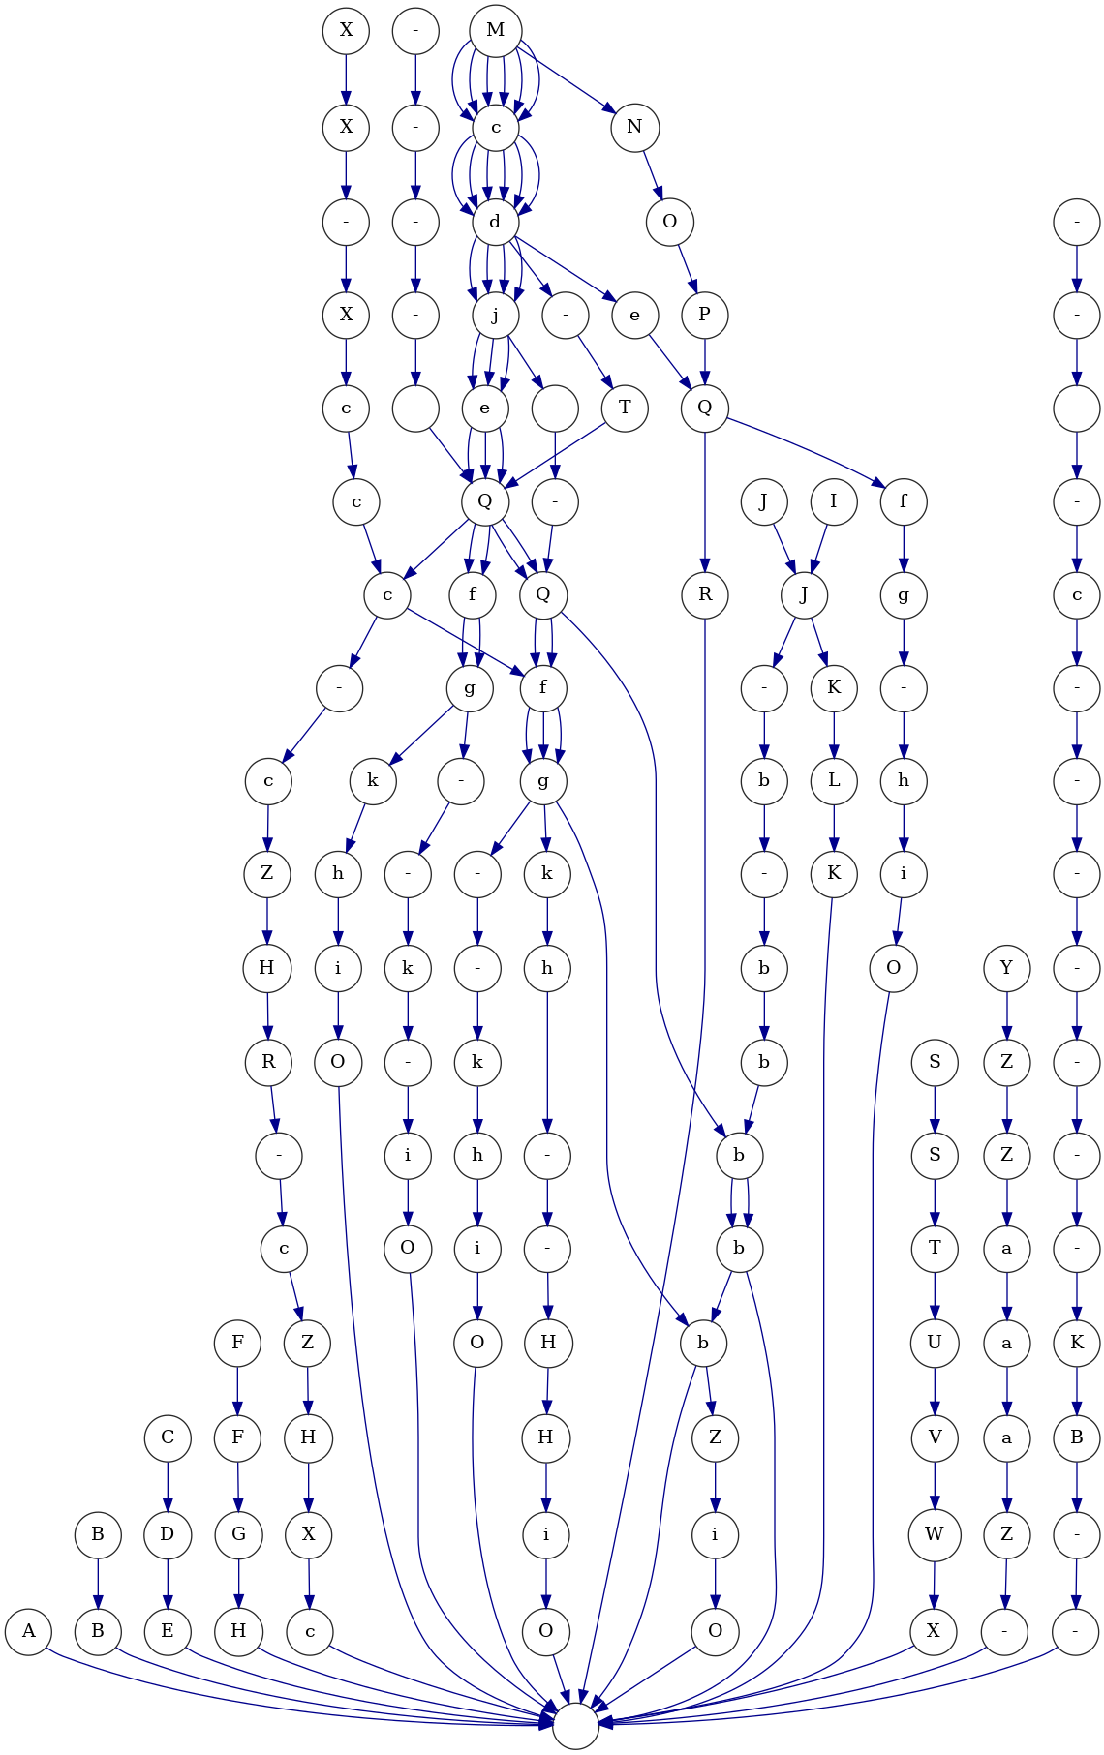
\includegraphics[width=0.8\linewidth]{Okamoto_fig/digraph-dtom.pdf}
        \vspace{-5mm}
	\caption{DtoMユーザの代表CTパスを可視化した状態遷移図}
	\label{fig:digraph-dtom}
\end{figure*}

\section{考察}

\subsection*{BtoDユーザ}

本分析は表\ref{tab:ranking-btod}に従い,BtoDユーザが習熟度向上の際に制作する作品のCTスコア重複数上位1件に属するユーザのみを抽出しているため,表\ref{tab:dict-btod}に示した本分析の対象ユーザが頻繁に獲得するCT概念が他ユーザのCTパスでも利用されるか調査した.結果として,表\ref{tab:dict-btod}の全てにおいて本分析の対象を除くユーザのCTパスでも各CT概念が最低873回以上獲得されていることが確認できた.したがって,本分析の結果は対象ユーザだけにとどまらず,全体のユーザに対しても当てはまることが示唆された.また,作品制作数を跨いで最多で出現したBのスキルについても本分析の対象を除くユーザのCTパスでの獲得回数を調査した.結果として,重複を含めて,1,966回獲得されていることが確認できた.BtoDユーザがCTスキルを獲得する回数の合計は20,558回であり,約10\%の確率でBtoDユーザはBのスキルを獲得することが示唆された.

\subsection*{DtoMユーザ}

本分析は表\ref{tab:ranking-dtom}に従い,DtoMユーザが習熟度向上の際に制作する作品のCTスコア重複数上位1件に属するユーザのみを抽出しているため,表\ref{tab:dict-dtom}に示した本分析の対象ユーザが頻繁に獲得するCT概念が他ユーザのCTパスでも利用されるかの調査をBtoDユーザ同様に行った.結果として,表\ref{tab:dict-dtom}の全てにおいて本分析の対象を除くユーザのCTパスでも各CT概念が最低23回以上獲得されていることが確認できた.したがって,本分析の結果は対象ユーザだけにとどまらず,全体のユーザに対しても当てはまることが示唆された.

\vspace{5mm}


考察として,これらの分析結果は,CTスキルの獲得過程が習熟度向上において非常に重要であることを強調している.異なる習熟度レベルや制作する作品数によって重要となるCTスキルのセットが異なるため,教育の設計においては,これらの違いを考慮に入れ,ユーザが適切なCTスキルを効果的に獲得できるよう支援する必要がある.

\chapter{RQ2:ユーザが獲得してきたCT7概念から次の作品でCT習熟度が向上するかどうかを予測することは可能か?}
\section{CT習熟度到達タイミングの予測}
本章ではユーザのCT獲得過程に基づいて,ユーザが次に制作する作品が特定の習熟度以上の評価を得るかを予測するモデルとして,習熟度到達予測モデルを構築し,従来モデルとの比較を行う.また,評価結果を基に,モデルの精度に寄与する要因と従来モデルとの予測結果の特徴の違いについて考察する.
\section{分析手法}
\subsection{CT習熟度到達予測モデルの構築}
従来研究より,目的変数の異なる2種類の予測モデルを構築する.

\begin{description}
\item [BtoDモデル:]CTスコアが8点以上(Developing以上)のオリジナル作品を制作するユーザを予測
\item [DtoMモデル:]CTスコアが15以上(Master)のオリジナル作品を制作するユーザを予測
\end{description}

目的変数は,{$N~(3 \leq N \leq 20)$}番目にDeveloping以上またはMasterに到達するオリジナル作品を制作したユーザを正例クラス,それ以外のユーザを負例クラスとする.例えば,BtoDモデルの構築では2番目以降に制作するオリジナル作品でDeveloping以上の評価を得るユーザを正例クラスとし,そうでないユーザを負例クラスとして扱う.また従来研究~\cite{Ando_2021}では,ユーザが目標の習熟度を満たす作品を1回でも制作すれば当該習熟度に到達すると判断しているため,本研究でも同様に扱う.構築するモデルでは,ユーザがオリジナル作品で目標習熟度以上のCTスコア合計点を獲得した場合のみ到達したと判断し,リミックス作品によるCTスコア合計点の獲得は目標習熟度に到達したと判定しない.また,N=1となる正例クラスは,特徴量として説明する作品数が0件となるため,モデルの構築時には除外する.

\ref{sec:3-analysis}節の結果より,BtoDユーザとDtoMユーザが作品制作過程で獲得するCT概念には特徴があったことから,従来モデルで用いた説明変数と本節で提案するCTパス重複数を考慮した説明変数を結合してモデルを学習する.

従来モデルでは,説明変数としてユーザが過去20作品を制作する中で使用したCT7概念の点数(0点から3点の4種類)までの獲得有無を用いた.また,従来研究\cite{Dasgupta_2016}よりリミックス作品の制作による学習効果も示されていることから,オリジナル作品とリミックス作品で獲得した点数を区別している.したがって,本実験でも従来研究と同様に$7(7つのCT概念) \times 4(0点から3点) \times 2(オリジナル作品またはリミックス作品)$の計56次元の説明変数を計測する.さらに本研究ではユーザの作品制作過程を捉えるための新しい説明変数を提案する.

本実験ではモデルの学習時にユーザの作品制作過程を考慮するため,ユーザが目標習熟度に次の作品で到達する確率としてパス遷移確率$P$を計測する.

まず,対象ユーザ群から\ref{sec:chapter_3-2}節と同様に,各ノード間のCTパス重複数を算出する.
パス遷移確率$P_{n,m}$は,ユーザが$n$番目に制作する作品から$m$番目に制作する作品,つまりノード$n$からノード$m$番目に到達する確率を意味し,式\ref{formula: single-ct-path}と式\ref{formula:ct-path}から算出する.ここで$N+1=\{ {n + 1}_1, {n + 1}_2,\ldots,{n + 1}_{k-1}, {n + 1}_k  \}$は,$n$の次に遷移するノード$n+1$の全体集合を意味し,式\ref{formula:ct-path}の分母はノード$n$からN+1に遷移するCTパス重複数の合計数である.

\begin{equation}
  B_n = \frac{nからn+1のCT
  パス重複数}{\sum_{j=1}^{k} (nからn+1_jのCTパス重複数)} \label{formula: single-ct-path}
\end{equation}

% \begin{equation}
%   P_n = B_n \times P_{n-1} (P_1 = B_1) \label{formula:ct-path}
% \end{equation}

\begin{equation}\label{formula:ct-path}
  P_{n,m} = B_m \times B_{m-1} \times \ldots \times B_{n+1} \times P_n \quad 
\end{equation}

本実験ではユーザの作品制作過程をモデルに反映するため,ユーザが制作する$n$番目の作品から$m$番目までの各パス遷移確率の集合$P_{i,i+1}|(n \leq i \leq m - 1)=\{P_{n,n+1}, P_{n+1,n+2}, \dots, P_{m-2, m-1}, P_{m-1, m}\}$を全て計測する.また,作品$m$は対象ユーザ群のうち,各ユーザが最後に制作した作品のひとつ前の作品とし,$n-m$の作品間ノード数$L$がモデルに与える影響も調査するため,作品$n$には$\{m-1, m-2,\dots, m-(L-1), m-L\}$を順に代入し,$P_{i,i+1}|(n \leq i \leq m - 1)$を算出する.この時,対象ユーザの作品数がLに満たない場合,そのユーザはモデルの学習から除外することとする.

本実験には,\ref{sec:chapter_3-1}節で収集したユーザ6,323人が1番目から20番目までに制作した作品126,460件を使用する.提案モデルの説明変数の計測には,最低限ユーザが3作品制作している必要があるため,ユーザ6,323人の中で3作品以上20作品以内の制作数を持つユーザ3,810人を対象とする.したがって,
CT概念獲得有無と,パス遷移確率$P$を結合した計$56+L \mid (1 \leq L \leq 18)$次元の説明変数を計測し,$L\mid (1 \leq L \leq 18)$個のBtoDモデル,DtoMモデルを構築する.

\subsection{機械学習アルゴリズム}
本論文では,ユーザの作品制作過程に基づく習熟度到達予測モデルの構築にランダムフォレスト~\cite{Breiman_2001}を用いる.ランダムフォレストとは,与えられた学習のデータから複数の決定木を作成し,それらを組み合わせてモデルを構築するアンサンブル学習法である.図\ref{fig:random-forest}にランダムフォレストの概要図を示す.ランダムフォレストは,まず与えられた学習データからランダムに復元抽出を行い,N個分の学習データ群を生成し,各決定木で予測を行う.最後に各決定木で出力された結果を多数決することにより,分類を行う.

本論文では,Pythonのscikit-learnを用いてランダムフォレストの実装を行う.ランダムフォレストのパラメータは従来研究との比較を行うために,作成する決定木の個数(図\ref{fig:random-forest})は200個,各決定木の作成に使用する特徴量の個数は各モデルの説明変数が持つ次元の平方根とする.また,クラス間の偏りを解消するため,モデル構築時に各クラスに出現する割合の逆数に基づいた重みづけを行う.例えば,対象ユーザが300人中,正例クラスが20人,負例クラスが280であった場合,それぞれのクラスの事例に300 / 20 = 15,300 / 280 = 1.07の重みを割り当てる.

\begin{figure*}[t]
	\centering
	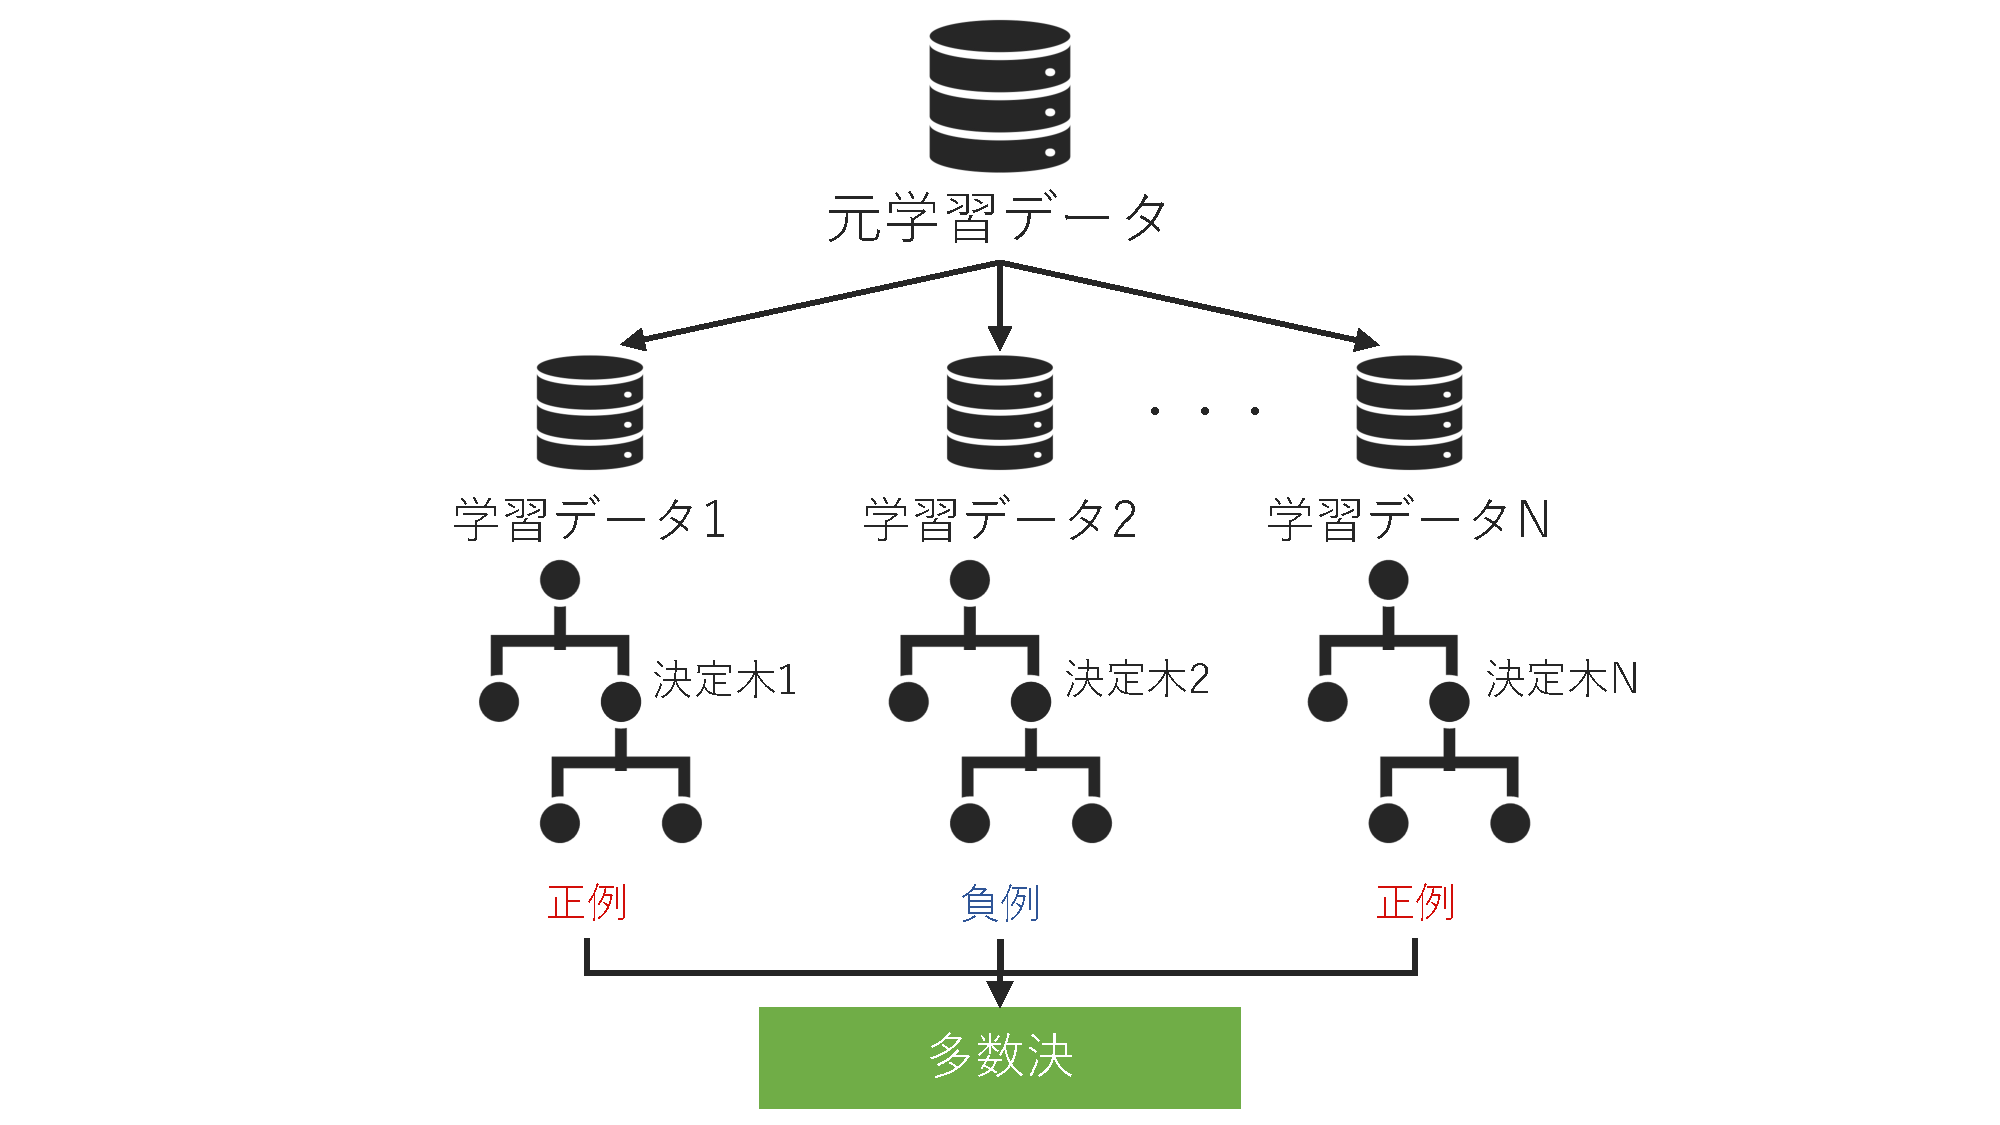
\includegraphics[width=1.0\linewidth]{Okamoto_fig/random-forest.pdf}
	\caption{ランダムフォレストの概略図}
	\label{fig:random-forest}
\end{figure*}

% \begin{table}
%   \caption{正例クラス,負例クラスに属するユーザ数の内訳}
%   \label{tab:user-class}
%   \vspace{2mm}
%   \centering
%   \begin{tabular}{c|c|c}
%     \hline
%      & 正例クラス & 負例クラス\\
%     \hline
%     \hline
%     モデル1 & 3,436人 & 1,108人 \\
%     \hline
%     モデル2 & 1,345人 & 4,800人 \\
%     \hline
%   \end{tabular}
% \end{table}

\subsection{モデルの評価方法}
本実験では,予測モデルの検証に従来研究と同じ層化K-分割交差検証を用いる.交差検証とは,モデルの構築時に使用するデータをK個に分割してK-1個を学習データ,残りの1個を検証データとして適用してK回繰り返すことで,予測モデルの汎化性能を評価する手法である.交差検証は,複数の学習データと検証データを組み合わせることで過学習(モデルが学習するデータには対応できるが,検証データには対応できない現象)の防止を実現する.

予測モデルの評価指標には適合率,再現率,F値を使用する.本研究で構築するモデルでは,ユーザが目標の習熟度に到達する(到達ユーザ)か到達していない(非到達ユーザ)かを予測するため,予測結果は以下の4つに分類できる.

\begin{description}
\item [True Positive(TP):]実際の到達ユーザに対して,到達ユーザであると正しく予測
\item [False Positive(FP):]実際の非到達ユーザに対して,到達ユーザであると誤って予測
\item [False Negative(FN):]実際の到達ユーザに対して,非到達ユーザであると誤って予測
\item [True Negative(TN):]実際の非到達ユーザに対して,非到達ユーザであると正しく予測
\end{description}

各評価指標は,上記の結果に基づいて算出される.適合率(Precision)は,式\ref{precision}に示すように予測モデルが到達ユーザと予測した内,実際に到達ユーザである割合を表す.

\begin{equation}
  適合率 = \frac{TP}{TP + FP} \label{precision}
\end{equation}
\vspace{.5mm}

再現率(Recall)は,式\ref{recall}で示すように到達ユーザの内,予測モデルにより正しく予測された到達ユーザの割合を表す.

\begin{equation}
  再現率 = \frac{TP}{TP + FN} \label{recall}
\end{equation}
\vspace{.5mm}

適合率と再現率は互いにトレードオフの関係にあるため,適合率,再現率の調和平均であるF値(F-measure)を用いる.F値は0から1の間の数値で算出され,値が高いほど予測モデルの精度が高いことを意味する.

\begin{equation}
  F値 = \frac{2 * 適合率 * 再現率}{適合率 + 再現率} \label{f-measure}
\end{equation}
\vspace{.5mm}

本研究では,交差検証によって10回の予測モデルの構築を行い,それぞれの予測結果で得られた3つの評価指標の平均値を算出し,評価を行う.

\subsection{特徴量重要度}

提案モデルで学習する説明変数(パス遷移確率$P$)が分類精度に与える影響を調査するために,予測モデルの精度向上に寄与する各説明変数の重要度を算出する.構築する予測モデルにおける説明変数\(f_{i}(1 \leq i \leq 56 + L \mid (1 \leq L \leq 18))\)の重要度\(importance_{f_{i}}\)は,説明変数\(f_{i}\)で分割したノードの集合を\(node_{f_{i}}\),ノードmの改善度を\(\triangle I_{m}\)とすると,式(\ref{equ:importance})のように表される.


% ------------------------------------------
% 式4.4 特徴量重要度の算出式
\begin{equation}
	\label{equ:importance}
	importance_{f_{i}}=\sum_{m\in node_{f_{i}}}\triangle{I_{m}}
\end{equation}
\vspace{0.5mm}
% ------------------------------------------


\noindent 重要度が高いとは,予測モデルの精度向上に大きく寄与することを意味しており,各説明変数の重要度の合計は1となる.しかし,本実験では層化10分割交差検証を使用して10個の予測モデルを構築するため,各説明変数の重要度はモデル構築ごとに異なる値を示す.そこで,10個のモデルにおける説明変数の重要度の順位を明らかにするために,順位傾向のクラスタ分析手法であるScott-Knott Effect Size Difference (ESD) 検定~\cite{Tantithamthavorn_2019}を用いる.Scott-Knott ESDは統計的に複数の点数をクラスタリングする手法であり,予測モデルに影響を及ぼす説明変数の特定にも広く使用されている.本実験では,10個の各予測モデルから得られる説明変数の順位を分類し,本実験で提案する説明変数の分類精度への影響度を確認する.

\section{実験結果}

本節では,2つの習熟度到達予測モデル(BtoDモデル,DtoMモデル)のうち,説明変数として与えるパスの長さ$L$毎の精度評価と,従来モデルとの精度比較,および分類精度に寄与する説明変数について述べる.

\subsection{モデルの分類精度}\label{subsec:model-result}

\begin{figure*}[t]
	\centering
	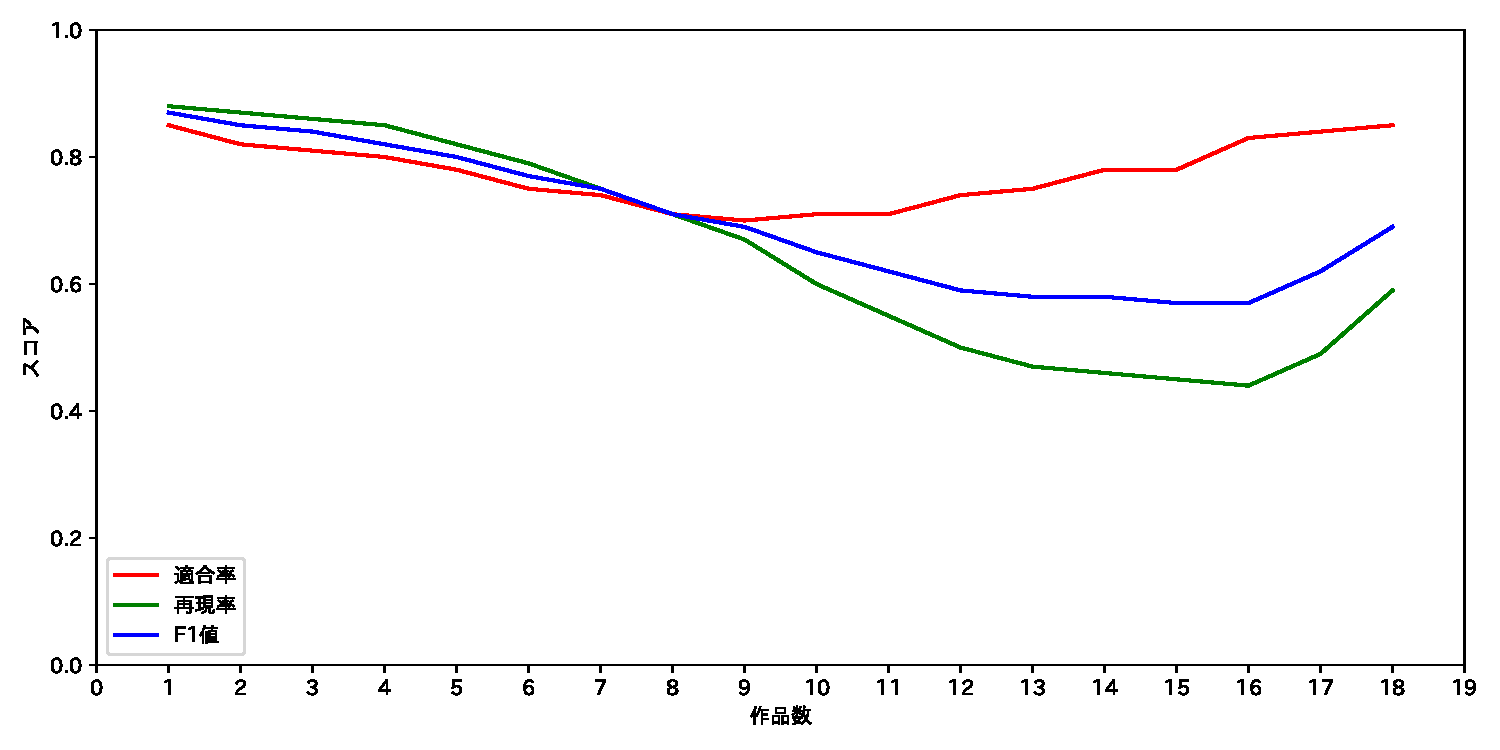
\includegraphics[width=1.0\linewidth]{Okamoto_fig/btod-lines2.pdf}
	\caption{提案BtoDモデルの作品数ごとの評価指標の遷移}
	\label{fig:btod-lines}
\end{figure*}

\begin{table}
  \caption{従来BtoDモデルと提案BtoDモデル(L=1)の精度比較}
  \label{tab:btod-model-comp}
  \vspace{2mm}
  \centering
  \begin{tabular}{l|c|c|c|c|c}
    \hline
     & 適合率 & 再現率 & F1値 & \begin{tabular}[c]{@{}c@{}}正確に予測できた\\BtoDユーザ数\end{tabular} & \begin{tabular}[c]{@{}c@{}}誤って予測された\\BtoDユーザ数\end{tabular}\\
    \hline
    \hline
    従来BtoDモデル & 0.84 & 0.86 & 0.85 & 2,333 & 370\\
    \hline
    提案BtoDモデル(L=1) & \textbf{0.85} & \textbf{0.88} & \textbf{0.87}  & 2,388 & 315\\
    \hline
  \end{tabular}
\end{table}


図\ref{fig:btod-lines}は,構築したBtoDモデルにおいて作品間ノード数$L$ごとの分類精度(適合率,再現率,F値)を示す.縦軸は評価スコア,横軸は作品間ノード数$L$を意味する.各分類精度は,層化10分割交差検証により出力した10回分の精度の平均値を表している.BtoDモデルの評価指標はノード数$L=1$のときに最も高い数値となり,適合率は0.85,再現率は0.88,F値は0.87であった.表\ref{tab:btod-model-comp}は従来BtoDモデルと提案BtoDモデルのうち,最も精度の高かったノード数$L=1$の分類精度と正しく予測されたBtoDユーザ数,誤って非BtoDユーザであると予測されたBtoDユーザ数を示す.従来BtoDモデルではDeveloping以上に到達したユーザに対して正しく予測できた数が2,333であるのに対し,提案BtoDモデルでは2,388であることから,提案BtoDモデルによって55人の習熟度向上ユーザが正しく予測できるようになったといえる.また,従来BtoDモデルではDeveloping以上に到達したユーザに対して到達していないと誤分類されたユーザ数が370であるのに対し,提案BtoDモデルでは315であることから,提案BtoDモデルによって55人のDeveloping以上に到達したユーザに対して誤分類が減ったといえる.従来BtoDモデルの適合率は0.84,再現率は0.86,F1値は0.85であり,提案BtoDモデルの適合率は0.85,再現率は0.88,F1値は0.87であることから,提案BtoDモデルは従来BtoDモデルと比べて適合率,再現率,F値において上回っているため,Developingに到達するユーザは直近に同じCT概念を持つ作品を制作することが多く,一度もDevelopingに到達しなかったユーザは直近に異なるCT概念を持つ作品を制作することが多いことが示唆される.

図\ref{fig:dtom-lines}は,構築したDtoMモデルにおいて作品間ノード数$L$ごとの分類精度(適合率,再現率,F値)を示す.縦軸は評価スコア,横軸は作品間ノード数$L$を意味する.各分類精度は,層化10分割交差検証により出力した10回分の精度の平均値を表している.BtoDモデルの適合率はノード数$L=9$のときに最も高い0.80となり,再現率,F値はノード数$L=1$のときに最も高くなり,それぞれ0.43,0.55であった.表\ref{tab:dtom-model-comp}は従来DtoMモデルと提案DtoMモデルのうち,最もF値が高かったノード数$L=1$の分類精度と習熟度が向上したと予測された非BtoDユーザ数を示す.従来DtoMモデルではMaster以上に到達したユーザに対して到達していないと誤分類されたユーザ数が207であるのに対し,提案DtoMモデルでは144であることから,提案DtoMモデルによって63人のMasterに到達しなかったユーザに対して誤分類が減ったといえる.従来DtoMモデルの適合率は0.70,再現率は0.44,F1値は0.54であり,提案DtoMモデルの適合率は0.77,再現率は0.45,F1値は0.59であった.従来DtoMモデルと比べて提案DtoMモデルは適合率,F値において上回っているため,BtoDモデルと同様に,Masterに到達するユーザは直近に同じCT概念を持つ作品を制作することが多く,一度もMasterに到達しなかったユーザは直近に異なるCT概念を持つ作品を制作することが多いことが示唆される.

\begin{figure*}[t]
	\centering
	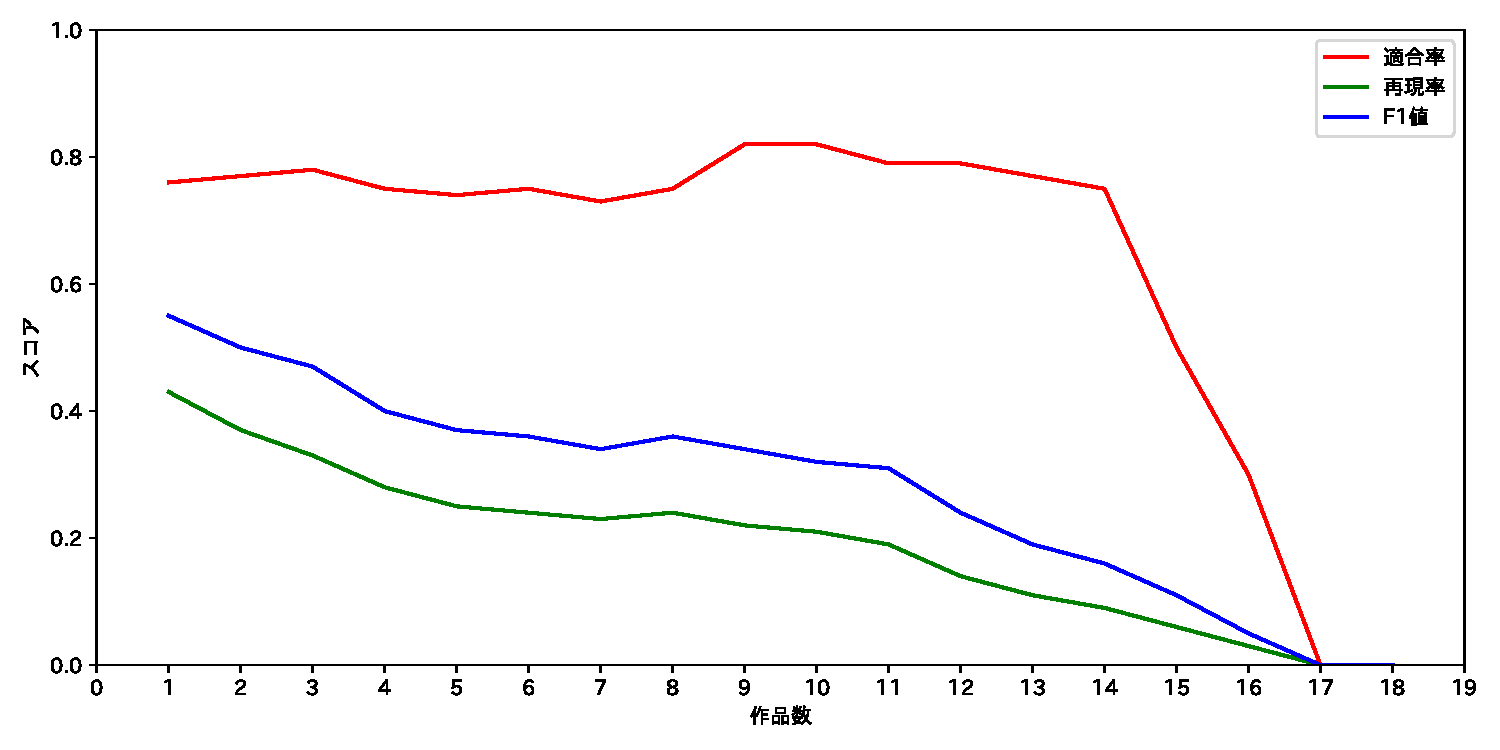
\includegraphics[width=1.0\linewidth]{Okamoto_fig/dtom-lines2.pdf}
	\caption{提案DtoMモデルの作品数ごとの評価指標の遷移}
	\label{fig:dtom-lines}
\end{figure*}

\begin{table}
  \caption{従来DtoMモデルと提案DtoMモデル(L=1)の精度比較}
  \label{tab:dtom-model-comp}
  \vspace{2mm}
  \centering
  \begin{tabular}{l|c|c|c|c}
    \hline
     & 適合率 & 再現率 & F1値 & \begin{tabular}[c]{@{}c@{}}誤って予測された\\非BtoDユーザ数\end{tabular}\\
    \hline
    \hline
    従来DtoMモデル & 0.70 & \textbf{0.44} & 0.54 & 207 \\
    \hline
    提案DtoMモデル(L=1) & \textbf{0.79} & \textbf{0.44} & \textbf{0.57} & 144 \\
    \hline
  \end{tabular}
\end{table}

\subsection{特徴量重要度}\label{subsec:importance}

\begin{table}[t]
    \caption{従来BtoDモデルと提案BtoDモデル(L=1)における重要度の高い説明変数の上位10件}\label{tab:feature_importance-btod}
    \centering
    \scalebox{0.85}{
        \begin{tabular}{r|rp{60mm}|rp{60mm}}
            \hline
            & \multicolumn{2}{c|}{従来BtoDモデル} & \multicolumn{2}{c}{提案BtoDモデル(L=1)} \\ \cline{2-5}
            グループ & \begin{tabular}{r} 重要度 \end{tabular} & \begin{tabular}{c} 説明変数 \end{tabular} & \begin{tabular}{r} 重要度 \end{tabular} & \begin{tabular}{c} 説明変数 \end{tabular} \\ \hline \hline
            1 & \begin{tabular}{r}0.05\end{tabular} & \begin{tabular}{r} \{オリジナル/フロー制御/0点\} \end{tabular} & \begin{tabular}{r} 0.20 \end{tabular} & \begin{tabular}{l} \{パス遷移確率P_{m-1,m} \} \end{tabular} \\ \hline
            2 & \begin{tabular}{r} 0.04 \end{tabular} & \begin{tabular}{r} \{リミックス/抽象化/0点\} \end{tabular} & \begin{tabular}{r} 0.04 \end{tabular} & \begin{tabular}{l} \{リミックス/データ表現/0点\} \end{tabular} \\ \hline
            3 & \begin{tabular}{r} 0.04 \end{tabular} & \begin{tabular}{r} \{オリジナル/データ表現/0点\} \end{tabular} & \begin{tabular}{r} 0.03 \end{tabular} & \begin{tabular}{l} \{オリジナル/ユーザ対話性/0点\} \end{tabular} \\ \hline
            4 & \begin{tabular}{r} 0.04 \end{tabular} & \begin{tabular}{r} \{オリジナル/ユーザ対話性/0点\} \end{tabular} & \begin{tabular}{r} 0.03 \end{tabular} & \begin{tabular}{l} \{オリジナル/フロー制御/0点\} \end{tabular} \\ \hline
            5 & \begin{tabular}{r} 0.04 \end{tabular} & \begin{tabular}{r} \{リミックス/並列/0点\} \end{tabular} & \begin{tabular}{r} 0.03 \end{tabular} & \begin{tabular}{l} \{リミックス/抽象化/2点\} \end{tabular} \\ \hline
            6 & \begin{tabular}{r} 0.04 \end{tabular} & \begin{tabular}{r} \{リミックス/データ表現/0点\} \end{tabular} & \begin{tabular}{r} 0.03 \end{tabular} & \begin{tabular}{l} \{リミックス/並列/0点\} \end{tabular} \\ \hline
            7 & \begin{tabular}{r} 0.04 \end{tabular} & \begin{tabular}{r} \{リミックス/抽象化/2点\} \end{tabular} & \begin{tabular}{r} 0.03 \end{tabular} & \begin{tabular}{l} \{オリジナル/データ表現/0点\} \end{tabular} \\ \hline
            8 & \begin{tabular}{r} 0.03 \end{tabular} & \begin{tabular}{r} \{リミックス/同期/0点\} \end{tabular} & \begin{tabular}{r} 0.03 \end{tabular} & \begin{tabular}{l} \{リミックス/抽象化/0点\} \end{tabular} \\ \hline
            9 & \begin{tabular}{r} 0.03 \end{tabular} & \begin{tabular}{r} \{リミックス/フロー制御/1点\} \end{tabular} & \begin{tabular}{r} 0.03 \end{tabular} & \begin{tabular}{l} \{リミックス/同期/0点\} \end{tabular} \\ \hline
            10 & \begin{tabular}{r} 0.03 \end{tabular} & \begin{tabular}{r} \{リミックス/論理/3点\} \end{tabular} & \begin{tabular}{r} 0.03 \end{tabular} & \begin{tabular}{l} \{リミックス/フロー制御/1点\} \end{tabular} \\ \hline
        \end{tabular}
    }
    \vspace{3mm}
\end{table}

\begin{table}[t]
    \caption{従来DtoMモデルと提案DtoMモデル(L=1)における重要度の高い説明変数の上位10件}\label{tab:feature_importance-dtom}
    \centering
    \scalebox{0.85}{
        \begin{tabular}{r|rp{60mm}|rp{60mm}}
            \hline
            & \multicolumn{2}{c|}{従来DtoMモデル} & \multicolumn{2}{c}{提案DtoMモデル(L=1)} \\ \cline{2-5}
            グループ & \begin{tabular}{r} 重要度 \end{tabular} & \begin{tabular}{c} 説明変数 \end{tabular} & \begin{tabular}{r} 重要度 \end{tabular} & \begin{tabular}{c} 説明変数 \end{tabular} \\ \hline \hline
            1 & \begin{tabular}{r} 0.04 \end{tabular} & \begin{tabular}{l} \{オリジナル/データ表現/0点\} \end{tabular} & \begin{tabular}{r} 0.12 \end{tabular} & \begin{tabular}{l} \{パス遷移確率P_{m-1,m}\} \end{tabular} \\ \hline
            2 & \begin{tabular}{r} 0.04 \end{tabular} & \begin{tabular}{r} \{オリジナル/抽象化/0点\} \end{tabular} & \begin{tabular}{r} 0.05 \end{tabular} & \begin{tabular}{l} \{オリジナル/同期/2点\} \end{tabular} \\ \hline
            3 & \begin{tabular}{r} 0.03 \end{tabular} & \begin{tabular}{r} \{オリジナル/同期/2点\} \end{tabular} & \begin{tabular}{r} 0.04 \end{tabular} & \begin{tabular}{l} \{オリジナル/抽象化/0点\} \end{tabular} \\ \hline
            4 & \begin{tabular}{r} 0.03 \end{tabular} & \begin{tabular}{r} \{オリジナル/フロー制御/3点\} \end{tabular} & \begin{tabular}{r} 0.03 \end{tabular} & \begin{tabular}{l} \{オリジナル/データ表現/0点\} \end{tabular} \\ \hline
            5 & \begin{tabular}{r} 0.03 \end{tabular} & \begin{tabular}{r} \{リミックス/同期/0点\} \end{tabular} & \begin{tabular}{r} 0.03 \end{tabular} & \begin{tabular}{l} \{リミックス/同期/0点\} \end{tabular} \\ \hline
            6 & \begin{tabular}{r} 0.03 \end{tabular} & \begin{tabular}{l} \{オリジナル/論理/0点\} \\ \{オリジナル/フロー制御/1点\} \\ \{リミックス/論理/0点\} \end{tabular} & \begin{tabular}{r} 0.03 \end{tabular} & \begin{tabular}{l} \{オリジナル/フロー制御/3点\} \end{tabular} \\ \hline
            7 & \begin{tabular}{r} 0.03 \end{tabular} & \begin{tabular}{r} \{オリジナル/並列/3点\} \end{tabular} & \begin{tabular}{r} 0.03 \end{tabular} & \begin{tabular}{l} \{オリジナル/並列/3点\} \end{tabular} \\ \hline
            8 & \begin{tabular}{r} 0.03 \end{tabular} & \begin{tabular}{r} \{オリジナル/同期/3点\} \end{tabular} & \begin{tabular}{r} 0.03 \end{tabular} & \begin{tabular}{l} \{オリジナル/データ表現/2点\} \end{tabular} \\ \hline
            9 & \begin{tabular}{r} 0.03 \end{tabular} & \begin{tabular}{r} \{リミックス/フロー制御/1点\} \end{tabular} & \begin{tabular}{r} 0.03 \end{tabular} & \begin{tabular}{l} \{オリジナル/並列/2点\} \\ \{リミックス/並列/0点\} \end{tabular} \\ \hline
            10 & \begin{tabular}{r} 0.03 \end{tabular} & \begin{tabular}{r} \{オリジナル/論理/2点\} \end{tabular} & \begin{tabular}{r} 0.03 \end{tabular} & \begin{tabular}{l} \{オリジナル/同期/3点\} \end{tabular} \\ \hline
        \end{tabular}
    }
    \vspace{3mm}
\end{table}

表\ref{tab:feature_importance-btod}と表\ref{tab:feature_importance-dtom}はそれぞれ従来BtoDモデルと提案BtoDモデル,従来DtoMモデルと提案DtoMモデルにおいて,分類精度に寄与した説明変数を重要度の高いグループ順に並び替えた結果を示す.重要度の値は,層化10分割交差検証により出力した10回分の重要度の平均値を示す.また,分類精度に寄与する説明変数はCT概念の場合,\{作品の種類/CT概念,点数\}のように示す.

表\ref{tab:feature_importance-btod}より,従来BtoDモデルでは,説明変数\{オリジナル/フロー制御/0点\}が分類精度に最も寄与し,続いて\{リミックス/抽象化/0点\},\{オリジナル/データ表現/0点\}が寄与しているのに対し,提案BtoDモデルでは本実験で提案した説明変数\{遷移確率$P_{m-1,m}$\}が分類精度に最も寄与し,続いて\{リミックス/データ表現/0点\},\{オリジナル/ユーザ対話性/0点\}が寄与していることがわかった.

表\ref{tab:feature_importance-dtom}より,従来DtoMモデルでは,説明変数\{オリジナル/データ表現/0点\}が分類精度に最も寄与し,続いて\{オリジナル/抽象化/0点\},\{オリジナル/同期/2点\}が寄与しているのに対し,提案BtoDモデルでは本実験で提案した説明変数\{遷移確率$P_{m-1,m}$\}が分類精度に最も寄与し,続いて\{オリジナル/同期/2点\},\{オリジナル/抽象化/0点\}が寄与していることがわかった.

従来BtoDモデルと従来DtoMモデルにおいて最も分類精度に寄与した説明変数と次に重要度の大きい説明変数との重要度の差はどちらも0.01程度であったが,提案BtoDモデルにおいて最も分類精度に寄与した\{遷移確率$P_{m-1,m}$\}の重要度は次に大きい\{リミックス/データ表現/0点\}の重要度の約5倍,また提案BtoDモデルにおいて最も分類精度に寄与した\{遷移確率$P_{m-1,m}$\}の重要度は次に大きい\{オリジナル/同期/2点\}の重要度の約2.4倍であることから,本提案モデルで用いた説明変数は予測に対して有効に働き,重要な指標であることが示唆される.


\section{考察}

本節では,構築した習熟度到達予測を行う従来モデルと提案モデルの評価結果に基づき,提案モデルの精度に起因する要因と,従来モデル,提案モデルで予測できた作品と予測できなかった作品とその特徴について考察する.

\subsection{提案モデルの精度に起因する要因}

\ref{subsec:model-result}節に示された通り,2種類の提案モデルに学習させる遷移確率$P$が1つの時に最高の精度を達成し,\ref{subsec:importance}節では,遷移確率$P$の特徴量重要度が高かったことから,特定の習熟度に到達するユーザと到達しないユーザ間では,作品M−1から作品Mへの遷移確率に差があることが示唆された.

図\ref{fig:add-btod}はDevelopingの習熟度に到達したユーザ(BtoDユーザ)とDevelopingに到達しなかったユーザ(非BtoDユーザ)が直前の作品に遷移する際のパスの重複数の分布を比較している.BtoDユーザの中央値は7.0,非BtoDユーザの中央値は3.0であり,Man-whitney U検定を実施したところ,統計的に有意な差(p$<$0.05)が確認できた.これは,Developingの習熟度に到達するユーザが頻繁に通るパスを辿るのに対し,到達しないユーザはあまり再現性のないパスを通っていることが示唆された.

また,図\ref{fig:add-dtom}はMasterの習熟度に到達したユーザ(DtoMユーザ)と,Developingに到達しなかったユーザ(非BtoDユーザ)が直前の作品に遷移する際のパスの重複数の分布を示す.DtoMユーザの中央値は2.0,非DtoMユーザの中央値は4.0であり,Man-whitney U検定を実施したところ,統計的に有意な差(p$<$0.05)を確認できた.Masterの習熟度に到達するユーザがより多様な作品から遷移する傾向にあること,また到達しないユーザはより再現性のあるパスを辿る傾向にあることを示している.


\begin{figure*}[t]
	\centering
	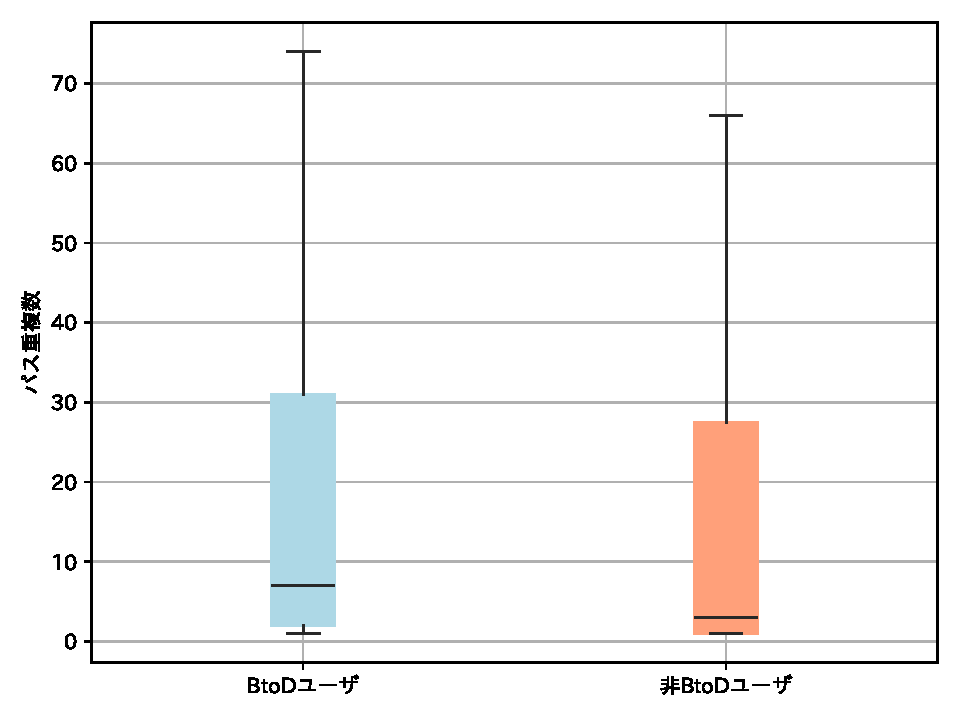
\includegraphics[width=0.7\linewidth]{Okamoto_fig/add-btod.pdf}
	\caption{BtoDユーザが直前の作品を制作する前のCTパス重複数}
	\label{fig:add-btod}
\end{figure*}

\begin{figure*}[t]
	\centering
	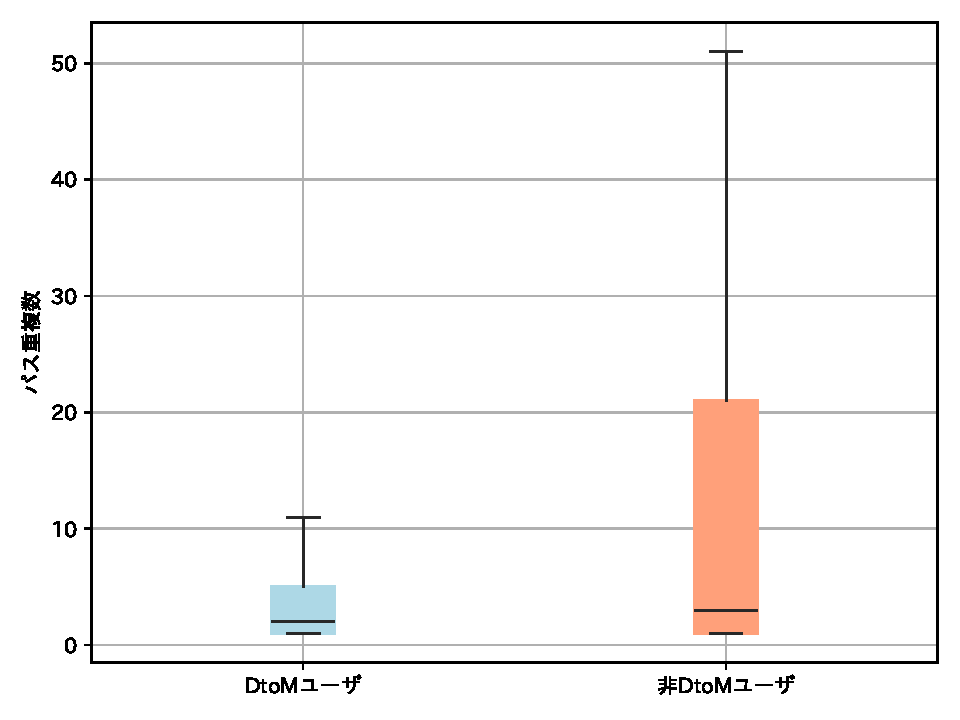
\includegraphics[width=0.7\linewidth]{Okamoto_fig/add-dtom.pdf}
	\caption{DtoMユーザが直前の作品を制作する前のCTパス重複数}
	\label{fig:add-dtom}
\end{figure*}



\subsection{従来モデルと提案モデルで予測できたユーザと予測できなかったユーザの特徴分析}

\subsubsection*{BtoDモデル}

図\ref{fig:btod-venn}に,従来BtoDモデルと提案BtoDモデルがそれぞれ予測できたユーザの数,両モデルが共に予測できたユーザの数,および予測できなかったユーザの数を示す.提案BtoDモデルでは,CTパスが同一で予測結果も一致したユーザのペアが12組見つかったが,従来BtoDモデルのみで予測できたユーザ内にはペアは見つからなかったことから,提案BtoDモデルによって作品制作過程を考慮した習熟度の到達予測が可能にしたことが示唆された.また,従来BtoDモデルと提案BtoDモデルで予測できたユーザは作品制作数の中央値が9.0であるのに対し,どちらのモデルでも予測できなかったユーザの作品制作数の中央値は19.0であった.Man-whitney U検定を実施したところ,統計的な有意差(p値$<$0.05)が確認できたことから,従来BtoDモデルと提案BtoDモデルでは作品制作数の多いユーザの作品制作過程は十分に考慮できておらず,分類が困難であることが示された.

\subsubsection*{DtoMモデル}

図\ref{fig:dtom-venn}に,従来DtoMモデルと提案DtoMモデルがそれぞれ予測できたユーザの数,両モデルが共に予測できたユーザの数,および予測できなかったユーザの数を示す.提案DtoMモデルで予測できたユーザの中でCTパスが同一で,予測結果が一致したユーザのペアは見つからなかった.このことから,\ref{sec:3-analysis}節で明らかにされた通り,DtoMユーザが多様なCTパスを通る傾向にあることを踏まえると,提案DtoMモデルでは作品制作過程を十分に考慮できていないことが示唆された.また,従来DtoMモデルと提案DtoMモデルで予測できたユーザは制作した作品数の中央値が17.0であるのに対し,どちらのモデルでも予測できなかったユーザが制作した作品数の中央値は11.0であった.Man-whitney U検定を実施したところ,統計的な有意差(p値$<$0.05)が確認できた.\ref{sec:3-analysis}節での分析により,DtoMユーザのうち,作品制作数が比較的少ないDtoMユーザの方がより多様性のあるCTパスを通る傾向にあることが明らかとなったことから,従来DtoMモデルと提案DtoMモデルでは作品制作数の比較的少ないユーザの作品制作過程は十分に考慮できていないことが示された.

\begin{figure*}[t]
	\centering
	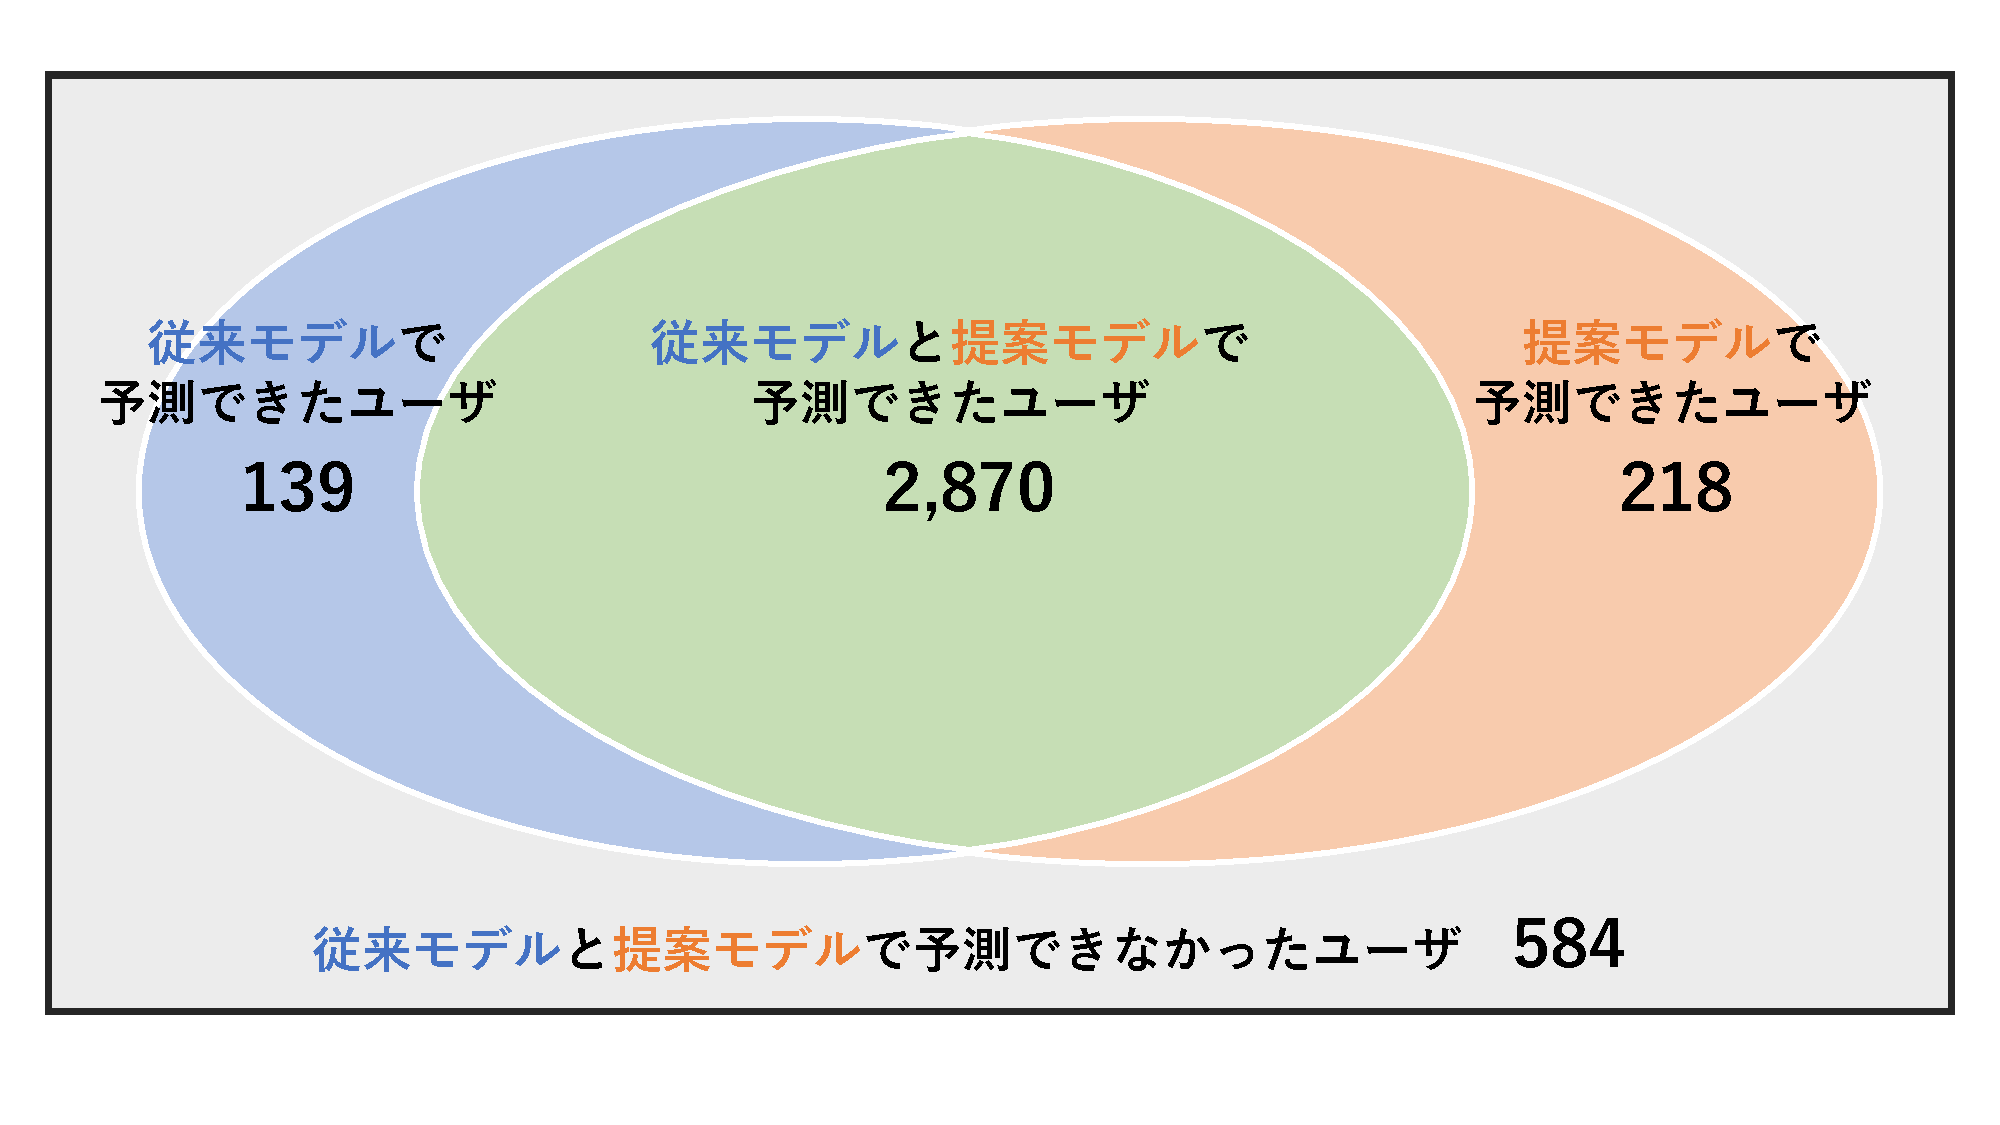
\includegraphics[width=1.0\linewidth]{Okamoto_fig/btod-venn.pdf}
        \vspace{-15mm}
	\caption{従来BtoDモデルと提案BtoDモデルで予測できたユーザと予測できなかったユーザ}
	\label{fig:btod-venn}
\end{figure*}

\begin{figure*}[t]
	\centering
	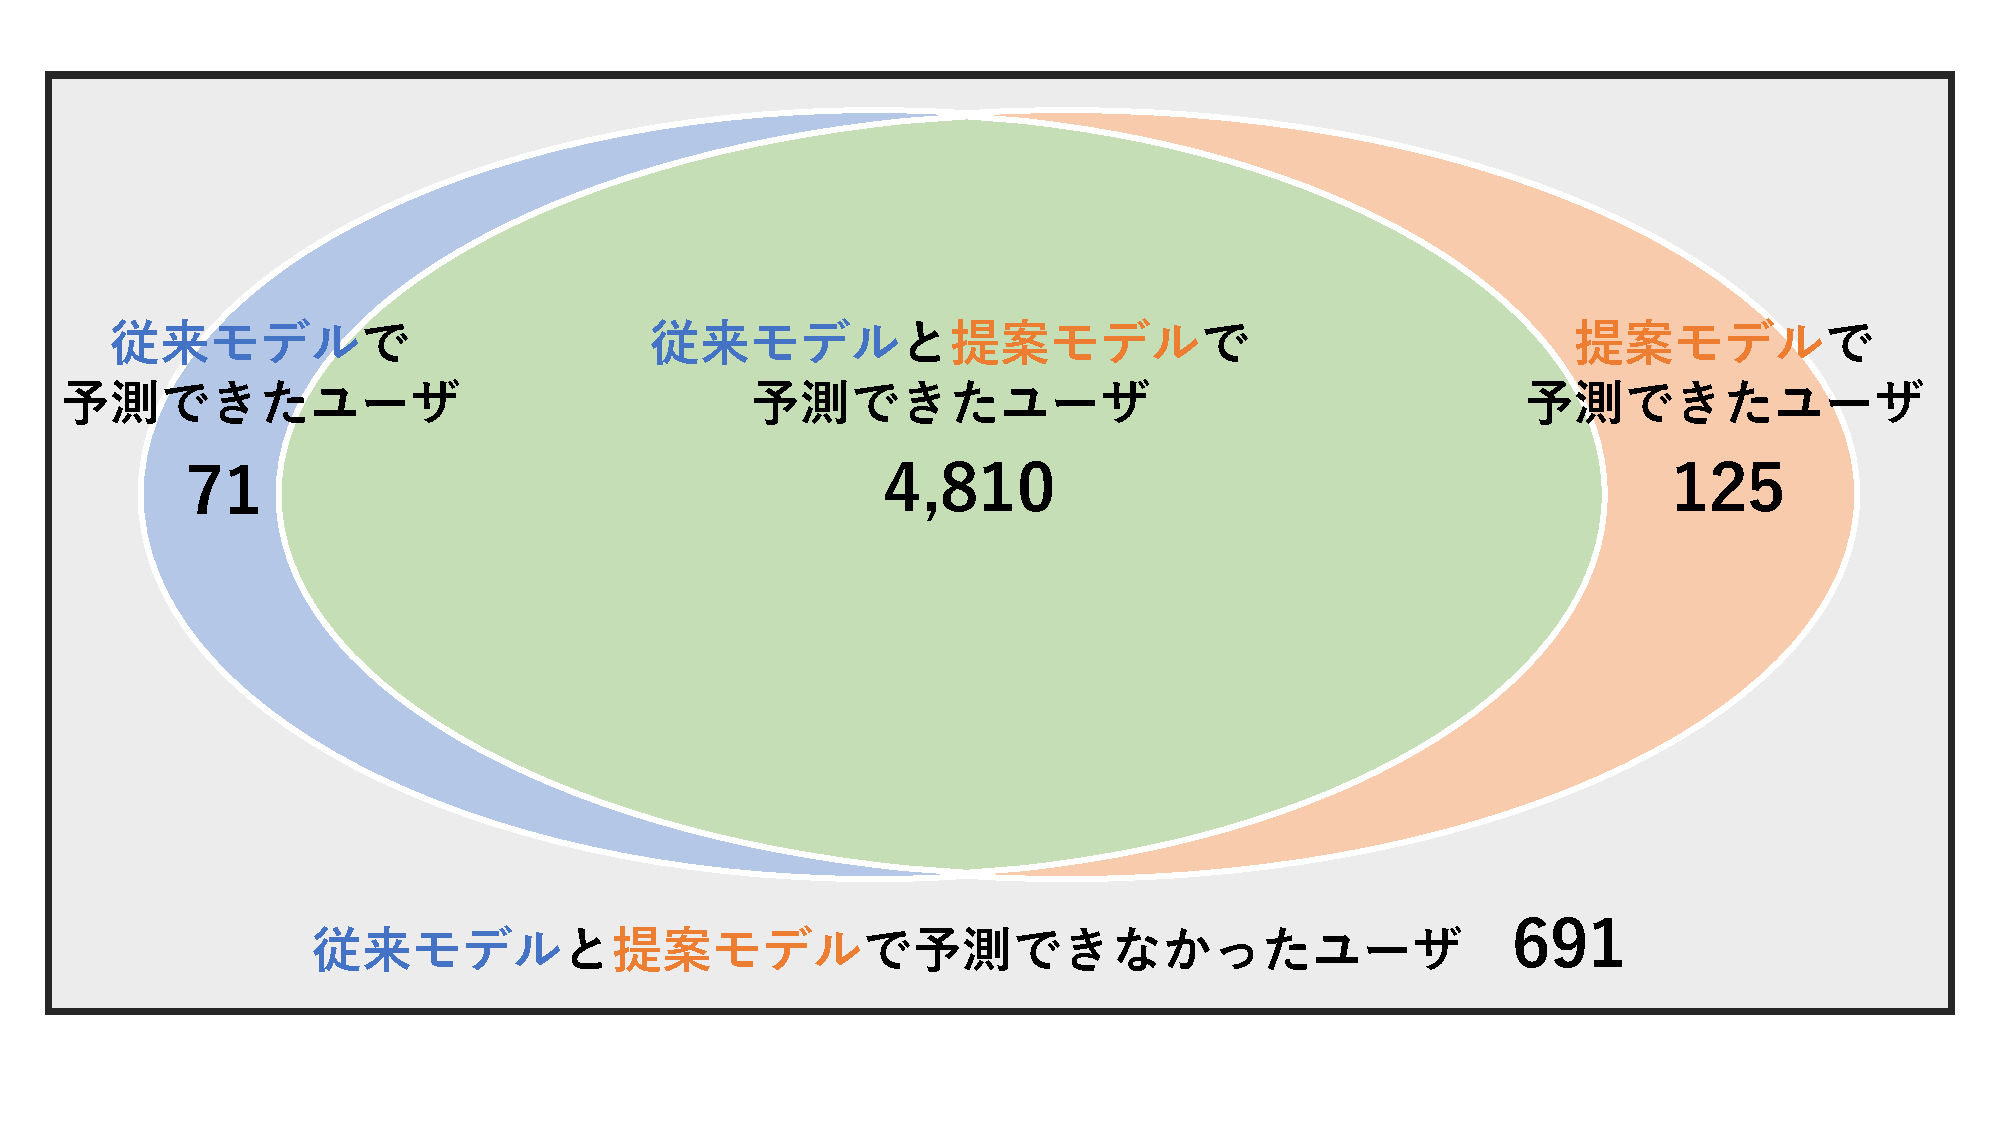
\includegraphics[width=1.0\linewidth]{Okamoto_fig/dtom-venn.pdf}
        \vspace{-15mm}
	\caption{従来DtoMモデルと提案DtoMモデルで予測できたユーザと予測できなかったユーザ}
	\label{fig:dtom-venn}
\end{figure*}



\chapter{妥当性への脅威}
\section{内的妥当性}

本論文では,ノード間の重複数をユーザの作品制作過程内の作品の重要な指標として捉えている.実際には,ユーザの作品制作過程の重要性を示す他の要因も存在することが考えられる.しかし,自由な作品制作環境下で,多くのユーザが複数回獲得されるCTスキルは作品制作過程において一定の重要性を持つと考える.

本論文では,ランダムフォレスト法を用いて習熟度到達予測モデルを構築した.構築した2つのモデルでは,正例クラスと負例クラスの数に偏りが存在したため,モデルの構築時に重みづけを行った.しかし,不均衡データの対応方法によってはモデルの予測精度に影響を与えることが考えられる.本論文では,層化10分割交差検証により,10個のモデルを構築した予測結果を用いることでその脅威を軽減する.

\section{外的妥当性}

本論文では,ユーザが実際にScratch上に公開する作品を基に習熟度到達予測モデルを構築した.その際にオリジナル作品の判断はScratch APIを用いて取得して情報を用いて行ったが,ユーザが他のユーザが制作した作品を模倣して制作する,あるいは他者に支援してもらい制作した作品が存在することも考えられる.これらの事例が対象ユーザに含まれている場合,分析結果やモデルの予測精度に違いが生じることが考えられるが,本論文ではユーザ6,323人が制作した作品126,460件を収集して多くの作品データを分析対象とすることで脅威を軽減する.




\chapter{おわりに}

本研究では,Scratchにおけるユーザのコンピュテーショナル・シンキング(CT)の作品制作過程に合わせた学習支援に向けて,まずユーザの作品制作過程の特徴を把握するために,ユーザが獲得してきたCT7概念の特徴量を分析した.分析の結果,BasicからDeveloping以上に到達するユーザの多くは同じCT概念の作品を繰り返し制作することが多く,共通して制作する作品があることがわかった.また,DevelopingからMasterに到達する多くのユーザは多様な作品を制作するものの,習熟度向上までに制作する作品数が多いユーザは共通したCT概念を持つ作品を制作することが多いことが明らかとなった.これらの分析結果を基に,ユーザの作品制作を考慮した説明変数を提案し,ユーザが次に特定の習熟度への到達するか否かを予測するモデルを構築して従来モデルとの比較を行った.結果として,提案モデルは従来モデルよりも精度が向上し,提案した説明変数がモデルの分類精度に最も影響を与えていることが明らかとなった.本研究により,ScratchにおけるユーザのCTスキル獲得状況に合わせた作品推薦等の学習支援の役立てとなることを期待する.

\begin{acknowledgements}

研究活動に取り組むにあたって多くの方々にご指導,ご協力を賜りました.ここにお世話になった方々への感謝の意を記させていただきます.

はじめに,指導教員である和歌山大学システム工学部伊原彰紀准教授に対し,厚く御礼申し上げます.研究室に配属して以来,研究の方針や,論文の執筆,発表資料制作において多くの時間を割いてご指導いただきました.また,対外発表の機会も設けていただいたことで,研究の面白さややりがいを知ることができ,多くの研究者と交流することで自身の研究に対する知見を深めることができました.先生のご尽力に敬意を表し,心より感謝いたします.

次に,和歌山大学システム工学研究科を修了された橋谷直樹氏並びに,和歌山大学システム工学部を卒業された三倉舞子氏,そしてソーシャルソフトウェア工学研究室の先輩方には,研究において多くのご指導とご助言をしていただきました.お忙しい中,研究内容の相談や,論文執筆についての支援だけでなく,大学生活においても大変お世話になりました.心より感謝いたします.

また,和歌山大学ソーシャルソフトウェア工学研究室並びに,オープンソースソフトウェア工学研究室の方々には,日頃から多大なるご協力と貴重なご助言をいただきましたこと,心より感謝いたします.特に,ソーシャルソフトウェア工学研究室の同期生の方々には,研究活動はもとより,大学生活全般にわたり,大変お世話になりました.時にはその存在が心の大きな支えとなっていました.深く感謝の意を表します.

最後になりましたが.日頃から暖かく見守っていただき,私を支えてくれた家族に対し,心より深く感謝いたします.

\end{acknowledgements}

%%%%%%%%%%%%%%%%%%%%%%%%%%%%%%%%%%%%%%%%%%%%%%%%%%%%%%%%%%%%%%%%%%%%%%%%

%%
%% 参考文献
%%

\bibliographystyle{junsrt}
\bibliography{Okamoto}

%%%%%%%%%%%%%%%%%%%%%%%%%%%%%%%%%%%%%%%%%%%%%%%%%%%%%%%%%%%%%%%%%%%%%%%%

%%
%% 付録
%%
% \appendix
% 
% \chapter{サンプルプログラム}
% 
% プログラムリストや実行結果など,本論を補足する上で必要と思われるものが
% あれば付録として付ける.
% 
% {
% \footnotesize
% \begin{verbatim}
% #include <stdio.h>
% int main(void)
% {
%     printf("Hello, World!\n");
%     return 0;
% }
% \end{verbatim}
% }

%%%%%%%%%%%%%%%%%%%%%%%%%%%%%%%%%%%%%%%%%%%%%%%%%%%%%%%%%%%%%%%%%%%%%%%%

\end{document}
